% Options for packages loaded elsewhere
\PassOptionsToPackage{unicode}{hyperref}
\PassOptionsToPackage{hyphens}{url}
\PassOptionsToPackage{dvipsnames,svgnames,x11names}{xcolor}
%
\documentclass[
  12pt,
  a4paperpaper,
  onecolumn]{article}

\usepackage{amsmath,amssymb}
\usepackage{lmodern}
\usepackage{iftex}
\ifPDFTeX
  \usepackage[T1]{fontenc}
  \usepackage[utf8]{inputenc}
  \usepackage{textcomp} % provide euro and other symbols
\else % if luatex or xetex
  \usepackage{unicode-math}
  \defaultfontfeatures{Scale=MatchLowercase}
  \defaultfontfeatures[\rmfamily]{Ligatures=TeX,Scale=1}
\fi
% Use upquote if available, for straight quotes in verbatim environments
\IfFileExists{upquote.sty}{\usepackage{upquote}}{}
\IfFileExists{microtype.sty}{% use microtype if available
  \usepackage[]{microtype}
  \UseMicrotypeSet[protrusion]{basicmath} % disable protrusion for tt fonts
}{}
\makeatletter
\@ifundefined{KOMAClassName}{% if non-KOMA class
  \IfFileExists{parskip.sty}{%
    \usepackage{parskip}
  }{% else
    \setlength{\parindent}{0pt}
    \setlength{\parskip}{6pt plus 2pt minus 1pt}}
}{% if KOMA class
  \KOMAoptions{parskip=half}}
\makeatother
\usepackage{xcolor}
\usepackage[left=2cm,top=1.5cm,right=2cm,bottom=1.5cm]{geometry}
\setlength{\emergencystretch}{3em} % prevent overfull lines
\setcounter{secnumdepth}{-\maxdimen} % remove section numbering
% Make \paragraph and \subparagraph free-standing
\ifx\paragraph\undefined\else
  \let\oldparagraph\paragraph
  \renewcommand{\paragraph}[1]{\oldparagraph{#1}\mbox{}}
\fi
\ifx\subparagraph\undefined\else
  \let\oldsubparagraph\subparagraph
  \renewcommand{\subparagraph}[1]{\oldsubparagraph{#1}\mbox{}}
\fi


\providecommand{\tightlist}{%
  \setlength{\itemsep}{0pt}\setlength{\parskip}{0pt}}\usepackage{longtable,booktabs,array}
\usepackage{calc} % for calculating minipage widths
% Correct order of tables after \paragraph or \subparagraph
\usepackage{etoolbox}
\makeatletter
\patchcmd\longtable{\par}{\if@noskipsec\mbox{}\fi\par}{}{}
\makeatother
% Allow footnotes in longtable head/foot
\IfFileExists{footnotehyper.sty}{\usepackage{footnotehyper}}{\usepackage{footnote}}
\makesavenoteenv{longtable}
\usepackage{graphicx}
\makeatletter
\def\maxwidth{\ifdim\Gin@nat@width>\linewidth\linewidth\else\Gin@nat@width\fi}
\def\maxheight{\ifdim\Gin@nat@height>\textheight\textheight\else\Gin@nat@height\fi}
\makeatother
% Scale images if necessary, so that they will not overflow the page
% margins by default, and it is still possible to overwrite the defaults
% using explicit options in \includegraphics[width, height, ...]{}
\setkeys{Gin}{width=\maxwidth,height=\maxheight,keepaspectratio}
% Set default figure placement to htbp
\makeatletter
\def\fps@figure{htbp}
\makeatother
\newlength{\cslhangindent}
\setlength{\cslhangindent}{1.5em}
\newlength{\csllabelwidth}
\setlength{\csllabelwidth}{3em}
\newlength{\cslentryspacingunit} % times entry-spacing
\setlength{\cslentryspacingunit}{\parskip}
\newenvironment{CSLReferences}[2] % #1 hanging-ident, #2 entry spacing
 {% don't indent paragraphs
  \setlength{\parindent}{0pt}
  % turn on hanging indent if param 1 is 1
  \ifodd #1
  \let\oldpar\par
  \def\par{\hangindent=\cslhangindent\oldpar}
  \fi
  % set entry spacing
  \setlength{\parskip}{#2\cslentryspacingunit}
 }%
 {}
\usepackage{calc}
\newcommand{\CSLBlock}[1]{#1\hfill\break}
\newcommand{\CSLLeftMargin}[1]{\parbox[t]{\csllabelwidth}{#1}}
\newcommand{\CSLRightInline}[1]{\parbox[t]{\linewidth - \csllabelwidth}{#1}\break}
\newcommand{\CSLIndent}[1]{\hspace{\cslhangindent}#1}

%----------------------------------------------------
% 	CONFIGURATION OF PARAMETERS
%----------------------------------------------------
% ----------------
%  FONTS AND TYPESETTING SETTINGS
% -----------------
\usepackage[english]{babel}
%\usepackage[bitstream-charter]{mathdesign}
%use\usepackage{times}
\usepackage{fontawesome5}
\usepackage{academicons}
\usepackage[notransparent]{svg}
\usepackage{tabu}
%\usepackage{coloremoji}
%\usepackage{emoji}

\usepackage{longtable}

%\usepackage[tracking=smallcaps]{microtype}
%\usepackage[bitstream-charter]{mathdesign}

% ----------------
%  STYLES OF THE CHAPTER, SECTION
% -----------------
%Options: Sonny, Lenny, Glenn, Conny, Rejne, Bjarne, Bjornstrup
%\usepackage[Bjornstrup]{fncychap}
\usepackage{marginnote}
\renewcommand*{\marginfont}{\small\sffamily}
\usepackage{wrapfig}
\usepackage{floatflt}
  
%---------------------------------
% Modification du model de UL
%\graphicspath{{./Figures/}} % chemin des figures


% -----------------
%  DEFINITION OF THE COLORS
% -----------------
%\usepackage{color} % Color
%\usepackage[usenames,dvipsnames,table]{xcolor}
%\usepackage{colortbl}

% -----------------
% 	MATHEMATHICAL SYMBOLS
% -----------------
%\usepackage{amssymb} %% The amssymb package provides various useful mathematical symbols
%\usepackage{amsthm} %% The amsthm package provides extended theorem environments
%\usepackage{amsmath}  % Paqute de Matematicas
%----------------------------------------------------------------------------------------

% -----------------
%  BIBLIOGRAPHY
% -----------------
%\usepackage  {natbib}
\usepackage{csquotes} %a utiliser si biblatex est utilisé
%\usepackage[style=numeric-comp, doi=false, backend=bibtex, isbn=false, url=false, sorting=none, language=english ]{biblatex}
%\addbibresource{library.bib}

%\usepackage[toc,page]{appendix}
\usepackage{booktabs}
% -----------------
%  VARIOUS PACKAGES FROM ME
% -----------------
%\usepackage{minitoc}
%\usepackage{booktabs} % Horizontal rules in tables
%\usepackage{float} % Required for tables and figures in the multi-column environment - they need to be placed in specific locations with the [H] (e.g. \begin{table}[H])
%\usepackage[lofdepth,lotdepth]{subfig} 
\usepackage{multirow} % Use multirows in the tables

%\usepackage {textcomp} % (Symbols Euros)
%\usepackage{nomencl} % nomenclature package
%\usepackage{soul}
%\renewcommand\thesection{\arabic{section}} %Redefinition of numeration of the document
%\usepackage{pdflscape} % hacer el documento lanscape en las hojas
%\usepackage{enumitem} % offers ready-made options for eliminating the space between items and paragraphs within the list (noitemsep) or all vertical spacing (nosep): 

\usepackage{enumitem}
\setlist[itemize]{noitemsep}

%\usepackage{afterpage} % For make blank pages
\usepackage{pdfpages} % For insert the title page.

\usepackage{mdframed}



% -----------------
%  VARIOUS PACKAGES FROM UNIVERSITE DE LORRAINE
% -----------------
%\usepackage{import}


%----------------------------------------------------------------------
%  PERSONALIZATION OF PACKAGES
%----------------------------------------------------------------------


% -----------------
%  DEFINITION OF COMMANDS BY ME
% -----------------
%\pagenumbering{Roman}






\usepackage{eurosym}

% To fix list things: 
\usepackage{enumitem}
\setitemize{noitemsep,topsep=0pt,parsep=0pt,partopsep=0pt,leftmargin=*}
\usepackage{amssymb}
\renewcommand{\labelitemi}{\tiny$\blacksquare$}

\usepackage{nopageno}




\usepackage{fancyhdr}
\pagestyle{fancy}
\renewcommand{\headrulewidth}{0pt} % Remove line at top
\setlength{\headheight}{14pt}

% Header
\lhead{\emph{Cruz Sanchez}} % Left of header
\chead{Part B1}
\rhead{DRAM Version 0.0.9}


% center of footer
%\fancyfoot[CO,CE]{And this is a fancy footer}
% page number on the left of even pages and right of odd pages
%\fancyfoot[LE,RO]{\thepage}
\cfoot{\thepage}

% 
% \newenvironment{itemize*}%
%   {\begin{itemize}%
%     \setlength{\itemsep}{0pt}%
%     \setlength{\parskip}{0pt}}%
%   {\end{itemize}}
% 

% 
\let\paragraph\oldparagraph
\let\subparagraph\oldsubparagraph
% 
\usepackage[compact]{titlesec}         % you need this package
\titlespacing{\subsubsection}{0pt}{3pt}{0pt} % this reduces space between (sub)sections to 0pt, for example
% \AtBeginDocument{%                     % this will reduce spaces between parts (above and below) of texts within a (sub)section to 0pt, for example - like between an 'eqnarray' and text
%   \setlength\abovedisplayskip{0pt}
%   \setlength\belowdisplayskip{0pt}}

\usepackage{indentfirst}
\setlength{\parindent}{15pt}% too much in my eyes delete this

\usepackage{lineno}
%\titleformat{\subsubsection}[block]{\hspace{2em}}{\thesubsubsection}{1em}{}
\makeatletter
\@ifpackageloaded{tcolorbox}{}{\usepackage[many]{tcolorbox}}
\@ifpackageloaded{fontawesome5}{}{\usepackage{fontawesome5}}
\definecolor{quarto-callout-color}{HTML}{909090}
\definecolor{quarto-callout-note-color}{HTML}{0758E5}
\definecolor{quarto-callout-important-color}{HTML}{CC1914}
\definecolor{quarto-callout-warning-color}{HTML}{EB9113}
\definecolor{quarto-callout-tip-color}{HTML}{00A047}
\definecolor{quarto-callout-caution-color}{HTML}{FC5300}
\definecolor{quarto-callout-color-frame}{HTML}{acacac}
\definecolor{quarto-callout-note-color-frame}{HTML}{4582ec}
\definecolor{quarto-callout-important-color-frame}{HTML}{d9534f}
\definecolor{quarto-callout-warning-color-frame}{HTML}{f0ad4e}
\definecolor{quarto-callout-tip-color-frame}{HTML}{02b875}
\definecolor{quarto-callout-caution-color-frame}{HTML}{fd7e14}
\makeatother
\makeatletter
\makeatother
\makeatletter
\makeatother
\makeatletter
\@ifpackageloaded{caption}{}{\usepackage{caption}}
\AtBeginDocument{%
\ifdefined\contentsname
  \renewcommand*\contentsname{Table of contents}
\else
  \newcommand\contentsname{Table of contents}
\fi
\ifdefined\listfigurename
  \renewcommand*\listfigurename{List of Figures}
\else
  \newcommand\listfigurename{List of Figures}
\fi
\ifdefined\listtablename
  \renewcommand*\listtablename{List of Tables}
\else
  \newcommand\listtablename{List of Tables}
\fi
\ifdefined\figurename
  \renewcommand*\figurename{Figure}
\else
  \newcommand\figurename{Figure}
\fi
\ifdefined\tablename
  \renewcommand*\tablename{Table}
\else
  \newcommand\tablename{Table}
\fi
}
\@ifpackageloaded{float}{}{\usepackage{float}}
\floatstyle{ruled}
\@ifundefined{c@chapter}{\newfloat{codelisting}{h}{lop}}{\newfloat{codelisting}{h}{lop}[chapter]}
\floatname{codelisting}{Listing}
\newcommand*\listoflistings{\listof{codelisting}{List of Listings}}
\makeatother
\makeatletter
\@ifpackageloaded{caption}{}{\usepackage{caption}}
\@ifpackageloaded{subcaption}{}{\usepackage{subcaption}}
\makeatother
\makeatletter
\@ifpackageloaded{tcolorbox}{}{\usepackage[many]{tcolorbox}}
\makeatother
\makeatletter
\@ifundefined{shadecolor}{\definecolor{shadecolor}{rgb}{.97, .97, .97}}
\makeatother
\makeatletter
\makeatother
\ifLuaTeX
  \usepackage{selnolig}  % disable illegal ligatures
\fi
\IfFileExists{bookmark.sty}{\usepackage{bookmark}}{\usepackage{hyperref}}
\IfFileExists{xurl.sty}{\usepackage{xurl}}{} % add URL line breaks if available
\urlstyle{same} % disable monospaced font for URLs
\hypersetup{
  colorlinks=true,
  linkcolor={blue},
  filecolor={Maroon},
  citecolor={Blue},
  urlcolor={blue},
  pdfcreator={LaTeX via pandoc}}

\author{}
\date{}

\begin{document}
\ifdefined\Shaded\renewenvironment{Shaded}{\begin{tcolorbox}[borderline west={3pt}{0pt}{shadecolor}, interior hidden, enhanced, breakable, sharp corners, frame hidden, boxrule=0pt]}{\end{tcolorbox}}\fi

\hypertarget{section-a-state-of-the-art-and-objectives}{%
\section{Section a: State of the art and
objectives}\label{section-a-state-of-the-art-and-objectives}}

\begin{tcolorbox}[enhanced jigsaw, toptitle=1mm, leftrule=.75mm, arc=.35mm, opacityback=0, left=2mm, titlerule=0mm, colbacktitle=quarto-callout-note-color!10!white, coltitle=black, bottomrule=.15mm, colframe=quarto-callout-note-color-frame, breakable, bottomtitle=1mm, title=\textcolor{quarto-callout-note-color}{\faInfo}\hspace{0.5em}{DRAM in a nutshell}, rightrule=.15mm, toprule=.15mm, colback=white, opacitybacktitle=0.6]
The main purpose of the Systemic Distributed Recycling via Open Hardware
(SDROM) is to establish a blueprint methodology for the design,
implementation and (e)valuation of micro-value chains of distributed
recycling at a urban territorial level. We seek to the achievement of a
three-level target: 1) Understand the establishment of a free-open
source technical ecosystem that can be printed, 2) to establish a set
indicators to possible help decision-makers and in the local
implementation of these initiatives in Europe/(America?), 3) \ldots..
\end{tcolorbox}

\hypertarget{section-a.-state-of-the-art-and-objectives}{%
\section{Section a. State-of-the-art and
objectives}\label{section-a.-state-of-the-art-and-objectives}}

\hypertarget{plastics-and-the-antropocene-a-change-is-needed}{%
\subsubsection{\texorpdfstring{\textbf{Plastics and the Antropocene: a
change is
needed}}{Plastics and the Antropocene: a change is needed}}\label{plastics-and-the-antropocene-a-change-is-needed}}

In the current paradigm, mass manufacturing plastic products are often
globalized value creation chains. The mass production system, in the
lens of deep
transition\textsuperscript{\protect\hyperlink{ref-kanger2022}{1}}
framework, is the fruit of a complex co-evolution of single unit
productions and interconnected systems that have intensified several
forms of environmental degradation without fully assuring the social
foundation's minimum standards (e.g.~healthcare, energy, water
etc)\textsuperscript{\protect\hyperlink{ref-raworth2017}{2}}. Thus, the
humanity is not only as biological but as geological force, on what is
recently considered as the Anthropocene
era\textsuperscript{\protect\hyperlink{ref-steffen2018}{3},\protect\hyperlink{ref-steffen2011}{4}}.
This new status of humanity is given the different indicators in the
natural ecosystems that are impacting the stability of the earth system.
For instance, the plastic waste contamination is one of the relevant
stratigraphic
indicator\textsuperscript{\protect\hyperlink{ref-porta2021}{5},\protect\hyperlink{ref-de-la-torre2021}{6}
}. More precisely, the soil and marine plastic pollution shows
ecological, biogeochemical and physical thresholds and they are becoming
a key component of the planetary
boundaries\textsuperscript{\protect\hyperlink{ref-raworth2017}{2},\protect\hyperlink{ref-ONeill2018}{7},\protect\hyperlink{ref-Rockstrom2009}{8}}
threat associated with chemical pollutants. Then, the use and disposal
of plastics is a societal problem characterized by high complexity and
multifaceted feedback loops that calls for a systemic view of the entire
plastics value chain from producers -petrochemical
companies-\textsuperscript{\protect\hyperlink{ref-Iles2013}{9},\protect\hyperlink{ref-DeVargasMores2018}{10}},
converters\textsuperscript{\protect\hyperlink{ref-Paletta2019}{11}},
brand owners or
manufacturers\textsuperscript{\protect\hyperlink{ref-Gong2020}{12},\protect\hyperlink{ref-Ma2020}{13}},
retailers and
consumers\textsuperscript{\protect\hyperlink{ref-Confente2020}{14}--\protect\hyperlink{ref-Filho2021}{16}},
and recycling
operators\textsuperscript{\protect\hyperlink{ref-Huysveld2019}{17},\protect\hyperlink{ref-Pazienza2020}{18}},
as well as the influences of policy-makers in wider economic and
societal
changes\textsuperscript{\protect\hyperlink{ref-Paletta2019}{11}}. The
delay that implies to put in place an alternative productive model is
the main the paradox in this issue. Therefore, how to manage the huge
amount of waste already present in the nature and the plastic waste
generated in the short term?, How to rethink production, consumption
systems (and even urban future cities) based on an engineering that is
concordance with the bio-geological cycles?, or What are alternative
trajectories for a socio-technical productive systems that take into
account the natural capital and
externalities\textsuperscript{\protect\hyperlink{ref-zhen2021}{19}}
since the fuzzy front-end design phase?. These major scientific
questions remains open towards a sustainable transition socio-technical
model.

\hypertarget{towards-circular-cities-a-promise-to-fullfill}{%
\subsubsection{Towards circular cities: a promise to
fullfill}\label{towards-circular-cities-a-promise-to-fullfill}}

Various schools of thought are proposing alternative socio-technical
manufacturing systems (and in some cases consumption), based on circular
economy\textsuperscript{\protect\hyperlink{ref-Murray2017}{20}},
bioeconomy, frugal innovation and degrowth. The circular economy concept
in the policy\textsuperscript{\protect\hyperlink{ref-EC2015}{21}},
industrial\textsuperscript{\protect\hyperlink{ref-EllenMacArthurFoundation2015}{22}}
and
scientific\textsuperscript{\protect\hyperlink{ref-nobre2021}{23}--\protect\hyperlink{ref-Schoggl2020}{25}}
arenas as an umbrella concept, but also as a contested
one\textsuperscript{\protect\hyperlink{ref-CalistoFriant2020}{26}--\protect\hyperlink{ref-corvellec2021}{28}}.
While the first two are not directly critical to capitalism and economic
growth, degrowth proponents argue that economic growth cannot be
sufficiently decoupled from environmental impacts, which renders further
growth of the economy unsustainable. Nevertheless, many cities have
taken up the resource management discourse to design circular economy
action plans, which aim to reduce urban environmental impacts while
generating new jobs, social well-being and room for innovation. Working
to make cities more circular implies adopting a particular approach,
using the concept of ``territorial metabolism,'' designating ``the set
of energy and material flows brought into play by the functioning of a
given
territory''\textsuperscript{\protect\hyperlink{ref-refBarles}{\textbf{refBarles?}}}.\\
This approach consists of understanding cities as the result of a
specific socio-ecological regime, no longer solely through their
functions or activities, but through their flows and stocks of materials
and resources. Indeed, cities worldwide are committed to becoming more
circular in their resource use, Looping actions ---reuse, recycling and
recovery of resources (materials, energy, water, land and
infrastructure)--- can help to address resource scarcity and wastage in
cities. However, whether or not their actions help them to reduce their
environmental impacts is
unclear\textsuperscript{\protect\hyperlink{ref-petit-boix2022}{29},\protect\hyperlink{ref-Petit-Boix2018}{30}}
and there are many challenges to implementation (Institutional,
Political, Regulatorial, Socio
Economical)\textsuperscript{\protect\hyperlink{ref-williams2019}{31}}.
Particularly, the key challengue lies in the bridging the boundaries of
urban planing and urban production systems a one coherent, continuum and
multi-scale design
process\textsuperscript{\protect\hyperlink{ref-Herrmann2020}{32}--\protect\hyperlink{ref-juraschek2022}{34}}.

\hypertarget{openess-for-design-global-manufacturing-local}{%
\subsubsection{Openess for `Design global / Manufacturing
local'}\label{openess-for-design-global-manufacturing-local}}

A major trend in the development of production systems seeks to
establish an urban production
model\textsuperscript{\protect\hyperlink{ref-Herrmann2020}{32},\protect\hyperlink{ref-juraschek2022}{34}}
with decentralized and distributed
characteristics\textsuperscript{\protect\hyperlink{ref-priavolou2022}{35},\protect\hyperlink{ref-cerdas2017}{36}}
as an alternative of globalized manufacturing values chains. Aiming at a
\emph{`design global / manufacturing local'}
(DGML)\textsuperscript{\protect\hyperlink{ref-Kostakis2018}{37}} seems a
proto-industrialization\textsuperscript{\protect\hyperlink{ref-sabel1985}{38}}
transition that is taking place in urban settlements that could a major
impact in the next short future. DGML is an emerging productive model
that builds on the convergence of the digital commons of knowledge,
software and design with local manufacturing technologies. More
precisely, the Open Source Appropriate Technology
(OSAT)\textsuperscript{\protect\hyperlink{ref-Pearce2010}{39}} and
peer-to-peer
(P2P)\textsuperscript{\protect\hyperlink{ref-Kostakis2013}{40}}
approaches have been seen potential drivers to propose an alternative
globalisation manufacturing
paradigm\textsuperscript{\protect\hyperlink{ref-Heikkinen2020a}{41}}.

The open source (OS) approach has become well-established to provide
improved product innovation over proprietary product
development\textsuperscript{\protect\hyperlink{ref-dibona1999}{42}--\protect\hyperlink{ref-deek2007}{45}}.
The evidence is most mature for software development because free and
open source software (FOSS) provides: i) diversification and open
innovation\textsuperscript{\protect\hyperlink{ref-colombo2014}{46}--\protect\hyperlink{ref-alexy2013}{48}},
ii) cumulative
innovation\textsuperscript{\protect\hyperlink{ref-boudreau2016}{49}},
iii) development
efficiency\textsuperscript{\protect\hyperlink{ref-hienerth2014}{50}},
iv) organizational
innovation\textsuperscript{\protect\hyperlink{ref-alexy2013}{48}}, v)
higher technical quality of
code\textsuperscript{\protect\hyperlink{ref-soderberg2015}{51}}, vi)
encourages
creativity\textsuperscript{\protect\hyperlink{ref-martinez2015}{52}} and
vii) perhaps most importantly, it avoids redundant
work\textsuperscript{\protect\hyperlink{ref-Ardal2016}{53}}. The OS
approach is now also gaining traction in free and open source hardware
(FOSH)\textsuperscript{\protect\hyperlink{ref-thompson2011}{54}--\protect\hyperlink{ref-li2018}{58}}
and appears to be roughly 15 years behind FOSS in development and
adoption\textsuperscript{\protect\hyperlink{ref-pearce2018}{59}}. One of
the primary drivers, is that all forms of free and open source
technology software and hardware (FOSS and FOSH) can provide a
substantial cost
savings\textsuperscript{\protect\hyperlink{ref-petch2014}{60}--\protect\hyperlink{ref-wittbrodt2013}{63}}.

The open source additive manufacturing technology, also know as 3D
printing, is playing a major role in the idea of democratization of
manufacturing
means\textsuperscript{\protect\hyperlink{ref-Beltagui2020}{64}}. In
particular, material extrusion based units are widely used, thanks to
the simplicity of operation, the Do-It-Yourself (DIY) approach and the
open-support communities. Thousands of open-source products are shared
by the global community from consumer goods to
scientific\textsuperscript{\protect\hyperlink{ref-Pearce2020a}{65}} and
medical
equipment\textsuperscript{\protect\hyperlink{ref-Pearce2020a}{65},\protect\hyperlink{ref-He2014}{66}}.
This model has been proven to be effective for emergency manufacturing
during the COVID-19
pandemic\textsuperscript{\protect\hyperlink{ref-Pearce2020a}{65},\protect\hyperlink{ref-tan2021}{67}}.
This is a driver communities to fabricate their own products for less
than the price of purchasing them. In that sense, the concept of urban
factory is evolving as a disruptive approach and is the materialization
of this manufacturing paradigm. The urban factory is defined as
``\emph{a factory located in an urban environment that is actively
utilizing the unique characteristics of its surroundings}''. It creates
products with a focus on the local market and allows customer
involvement during value
creation\textsuperscript{\protect\hyperlink{ref-Herrmann2020}{32},\protect\hyperlink{ref-Ijassi2022}{68}}.

\hypertarget{major-long-vision-convivial-urban-production}{%
\subsubsection{Major long vision: Convivial urban
production}\label{major-long-vision-convivial-urban-production}}

Today, a major societal issue rely on how to conceived socio-technical
`circular units' for manufacturing that integrates values of
sobriety\textsuperscript{\protect\hyperlink{ref-ref}{\textbf{ref?}}},
resilience\textsuperscript{\protect\hyperlink{ref-touriki2021}{69},\protect\hyperlink{ref-VanFan2019}{70}},
adaptability\textsuperscript{\protect\hyperlink{ref-weichhart2021}{71}}
and evolutive in urban settlements. The technologies that tend to lean
towards sufficiency and creativity; adopt the open-source philosophy;
are designed for affordability and durability; explore tacit knowledge;
empower communities through access to means of production; and promote
localisation of production and logistics; are defined as
\textbf{convivial}\textsuperscript{\protect\hyperlink{ref-priavolou2022}{35}}.
Moreover, the reuse, repairing, recycling approaches will need to
converge in a post-growth economy context considering the societal
issues of resource scarcity and waste accumulation in the urban
settlements\textsuperscript{\protect\hyperlink{ref-kallis2018}{72},\protect\hyperlink{ref-savini2021}{73}}.
Indeed, today the establishment of these socio-technical systems need to
include all ecosystem externalitites and the carrying capacity of the
ecosystem to claim to
sustainability\textsuperscript{\protect\hyperlink{ref-Bakshi2018}{74},\protect\hyperlink{ref-Bakshi2019a}{75}}.
The trend is reinforced by the fact that by 2050, it is expected that
about 70\% of the world's population will live in urban
settlements\textsuperscript{\protect\hyperlink{ref-savini2021}{73}}.
Urban cities will be responsible for non-negligible environmental
impact\textsuperscript{\protect\hyperlink{ref-Zheng2020}{76},\protect\hyperlink{ref-Sodiq2019}{77}},
producing about 50\% of global waste, and 75\% of greenhouse gas
emissions which affects the sustainability of
cities\textsuperscript{\protect\hyperlink{ref-schraven2021}{78}} and the
quality of city
life\textsuperscript{\protect\hyperlink{ref-Riffat2016}{79}}.

\hypertarget{distributed-recycling-via-additive-manufacturing-a-promising-inclusion}{%
\subsubsection{Distributed recycling via additive manufacturing: a
promising
inclusion}\label{distributed-recycling-via-additive-manufacturing-a-promising-inclusion}}

Since 2014, I have been working on the validation of the open-source 3D
printing,
filament-\textsuperscript{\protect\hyperlink{ref-CruzSanchez2014}{80}}
and
pellet-based\textsuperscript{\protect\hyperlink{ref-Arthur2020}{81}}, as
a robust manufacturing system, but also as a potential enabler of the
mechanical
recycling\textsuperscript{\protect\hyperlink{ref-Cruz2015}{82}--\protect\hyperlink{ref-lopez2022}{84}}
of plastic waste feedstock. Likewise, I have been working on the design
of the pertinent closed-loop supply
chain\textsuperscript{\protect\hyperlink{ref-Pavlo2018}{85},\protect\hyperlink{ref-Santander2020}{86}},
considering the applicable sustainability
indicators\textsuperscript{\protect\hyperlink{ref-Santander2022}{87}}
based on the scientific literature. In a recent
paper\textsuperscript{\protect\hyperlink{ref-CruzSanchez2020}{88}}, I
could establish \emph{distributed recycling for additive manufacturing
(DRAM)} as a theoretical model a great to possible recycling locally.
DRAM (See Figure~\ref{fig-DRAM}) is a breakthrough promise in the
constitution of a micro-circular industry units to validate the
technical feasibility, and several technological pathways are maturing
to allow individuals to recycle waste plastic directly by 3D-printing it
into valuable products.

\begin{figure}

{\centering 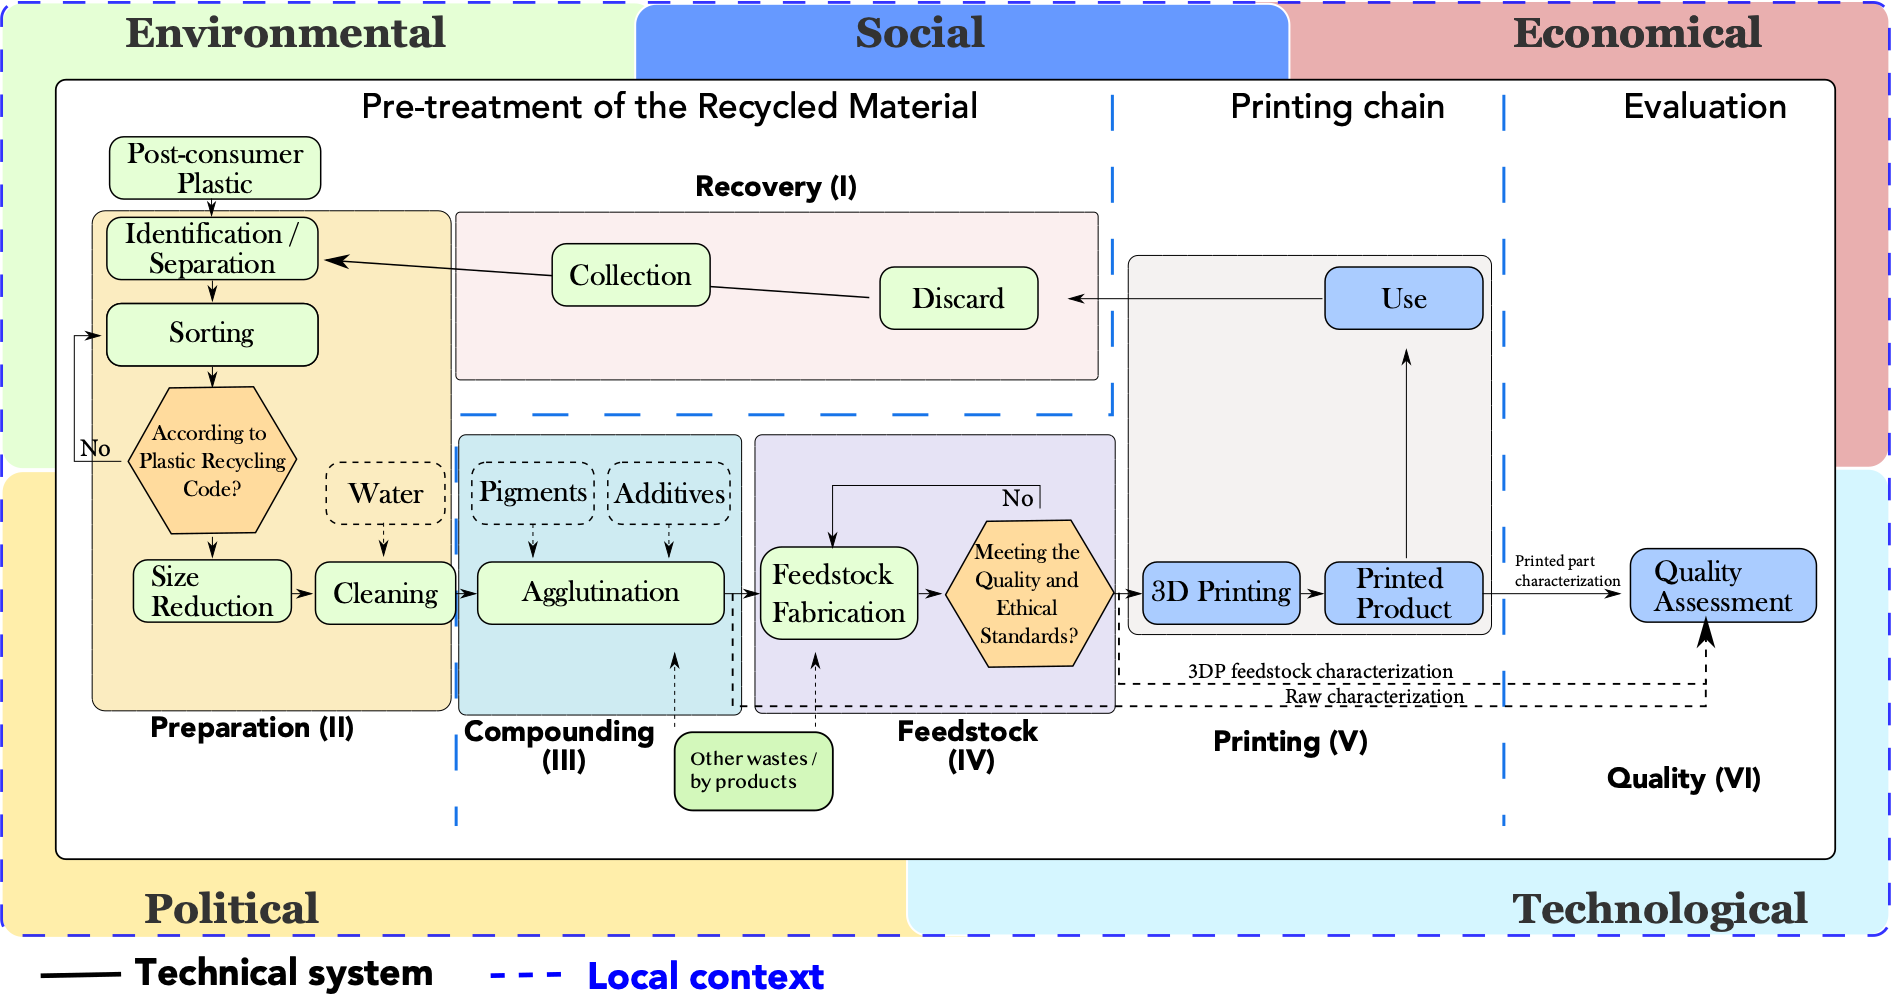
\includegraphics[width=0.9\textwidth,height=\textheight]{Figures/SDRAM-00.png}

}

\caption{\label{fig-DRAM}Distributed recycling via additive
manufacturing. Source}

\end{figure}

To appreciate the ground-breaking scientific nature of this idea, let me
state that historically, the plastic recycling has been oriented to
centralized facilities in order to take advantage of economies of scale
through the production of low-value products. However, it is proved to
be an expensive process due to the inherent separate collection,
transportation, processing and
remanufacturing\textsuperscript{\protect\hyperlink{ref-Hopewell2009}{89},\protect\hyperlink{ref-Singh2017b}{90}}.
Plastic production increased at compound annual growth rate of 8.4\%,
passing from \(2Mt\) in 1950 to \(368Mt\) in 2019, but the statistics
proves that only 9\% have been recycled while 79\% was accumulated in
landfills or the natural
environment\textsuperscript{\protect\hyperlink{ref-Geyer2017}{91}}.
\textbf{We need other paradigm to tackle this wicked problem}.

On the other hand, DRAM can starts with local plastic waste that is
produced everywhere from packaging to broken products (\emph{Recovery
(I)}). It is washed, dried and then ground or cut into particles using a
waste plastic granulator or office shredder (\emph{Preparation (II)}).
The raw material for FFF can be manufactured economically using
distributed means with a waste plastic extruder (often called a
``recyclebot'')\textsuperscript{\protect\hyperlink{ref-Baechler2013}{92}}
for mono or composite materials (\emph{Compounding (II) and Feedstock
(IV)}). Filament made with a recyclebot costs less than 10 cents per kg,
whereas commercial filament costs \$20/kg or more. This can produce
valuable products at remarkably low costs. For example, using a
recyclebot/3D-printer combination can produce over 300 units (e.g.,
camera lens hoods) for the price of one such item listed on marketplaces
(e.g.~Amazon). Fused granular fabrication is a recent experimental
approach enabling the printing process directly from
pellets\textsuperscript{\protect\hyperlink{ref-JustinoNetto2021}{93},\protect\hyperlink{ref-netto2022}{94}},
which reduces the degradation cycles of the plastic. For this process, I
worked in the desktop
format\textsuperscript{\protect\hyperlink{ref-Arthur2020}{81}}, but it
seems that this technology could further expand the boundaries of
additive manufacturing and eventually
recycling\textsuperscript{\protect\hyperlink{ref-billah2021}{95}--\protect\hyperlink{ref-Byard2019}{97}}
for larger
object\textsuperscript{\protect\hyperlink{ref-petsiuk2022}{98}}.
Distributed recycling fits into the circular economy
paradigm\textsuperscript{\protect\hyperlink{ref-Zhong2018}{99}--\protect\hyperlink{ref-Despeisse2016}{101}},
as it eliminates most embodied energy and pollution from transportation
between processing steps. Also, it decreases the embodied energy of
filament by 90\% compared to traditional centralized filament
manufacturing using fossil fuels as
inputs\textsuperscript{\protect\hyperlink{ref-Kreiger2013}{102}--\protect\hyperlink{ref-Horta2017}{104}}.
Additionally, open-source investment should result in an extremely high
return on investment
(ROI)\textsuperscript{\protect\hyperlink{ref-Pearce2020a}{65}}. This
makes distributed recycling environmentally superior to other methods of
plastic recycling systems.

However, major efforts in the scientific literature have been only
concentrated in the materials and technical validation in laboratory
conditions. \textbf{The analysis of the holistic impact that this
process can have in the context of a city remains not well understood}.
From the urban planning perspective, there are not methodological tools
to (e)valuate (to see the impact but also to see the worth) of possible
distributed plastic networks supported by the open source. Indeed, a
community-driven of plastic recycling remains in the makers, Fablabs
spheres where the competences and values may differe from the general
public. A system validation is needed to possible understant the
pertinent scale that his approach can take in urban settlements.

In the framework of a EUH2020 project called INEDIT\footnote{See
  https://cordis.europa.eu/project/id/869952}, I have been leading the
implementation of the \textbf{Green Fablab} demostrator inside the third
place called Octroi-Nancy Association \footnote{See
  https://www.octroi-nancy.fr/} since November 2021\footnote{This
  demostrator found retard because of the pandemic situation.}. INEDIT
project aims to create an ecosystem to transform the DYI practices
largely documented in FabLabs/Hacker/Maker spaces into a professional
approach called Do-It-Together to capitalise on the knowledge,
creativity and ideas of design and engineering. The Green Fablab is a
distributed recycling demonstrator that use living lab
approach\textsuperscript{\protect\hyperlink{ref-tyl2021}{105},\protect\hyperlink{ref-compagnucci2020a}{106}}
to experiment in real conditions with citizens, final users and large
general public. This experiment is enframed as a design for
sustainability at a socio-technical system
level\textsuperscript{\protect\hyperlink{ref-Ceschin2016}{107}}. We have
collected and recycling around 100kg of plastic waste for the
pedagogical and architectural uses given the fact that we are connected
with a creative ecosystem of designers and makers participatin in the
Octroi-Nancy projet. This hands-on experience confirms the literature
that a new recycled resources industry is starting to conceived inside
the cities\textsuperscript{\protect\hyperlink{ref-wang2019b}{108}}. This
industry is seen as driver consists of a series of activities related to
recycled resources -- e.g., recycling, refining, remanufacturing, etc.
-- aspiring to mitigate the negative externality caused by the linear
economy. The signal RRI has thus been highlighted on many countries'
agendas to promote the circular
society\textsuperscript{\protect\hyperlink{ref-leipold2021}{109}--\protect\hyperlink{ref-jaeger-erben2021a}{111}}.
In the case of plastic waste, the main difficulty remains to make
affordable the use of new secondary material applicability by the
industry\textsuperscript{\protect\hyperlink{ref-klotz2022}{112}}, but
more profoundly, how these new socio-technical technical systems will
interact with the urban planning process and policymaking to make
concrete the ambition of circularity inside the urban settlements.

\hypertarget{ambition-objectives}{%
\subsection{2. Ambition \& objectives}\label{ambition-objectives}}

The material'
rarefaction\textsuperscript{\protect\hyperlink{ref-hultman2021}{113}},
the need for ecological integration of manufacturing
systems\textsuperscript{\protect\hyperlink{ref-Bakshi2019a}{75},\protect\hyperlink{ref-Bakshi2015}{114},\protect\hyperlink{ref-Saladini2018}{115}}
and the urban
resilience\textsuperscript{\protect\hyperlink{ref-xu2021e}{116}} calls
for pushing forward the boundaries of knowledge of the design of urban
production systems to unleash a sustainability transition.

\begin{wrapfigure}[13]{r}[0pt]{0.45\textwidth}
\centering
    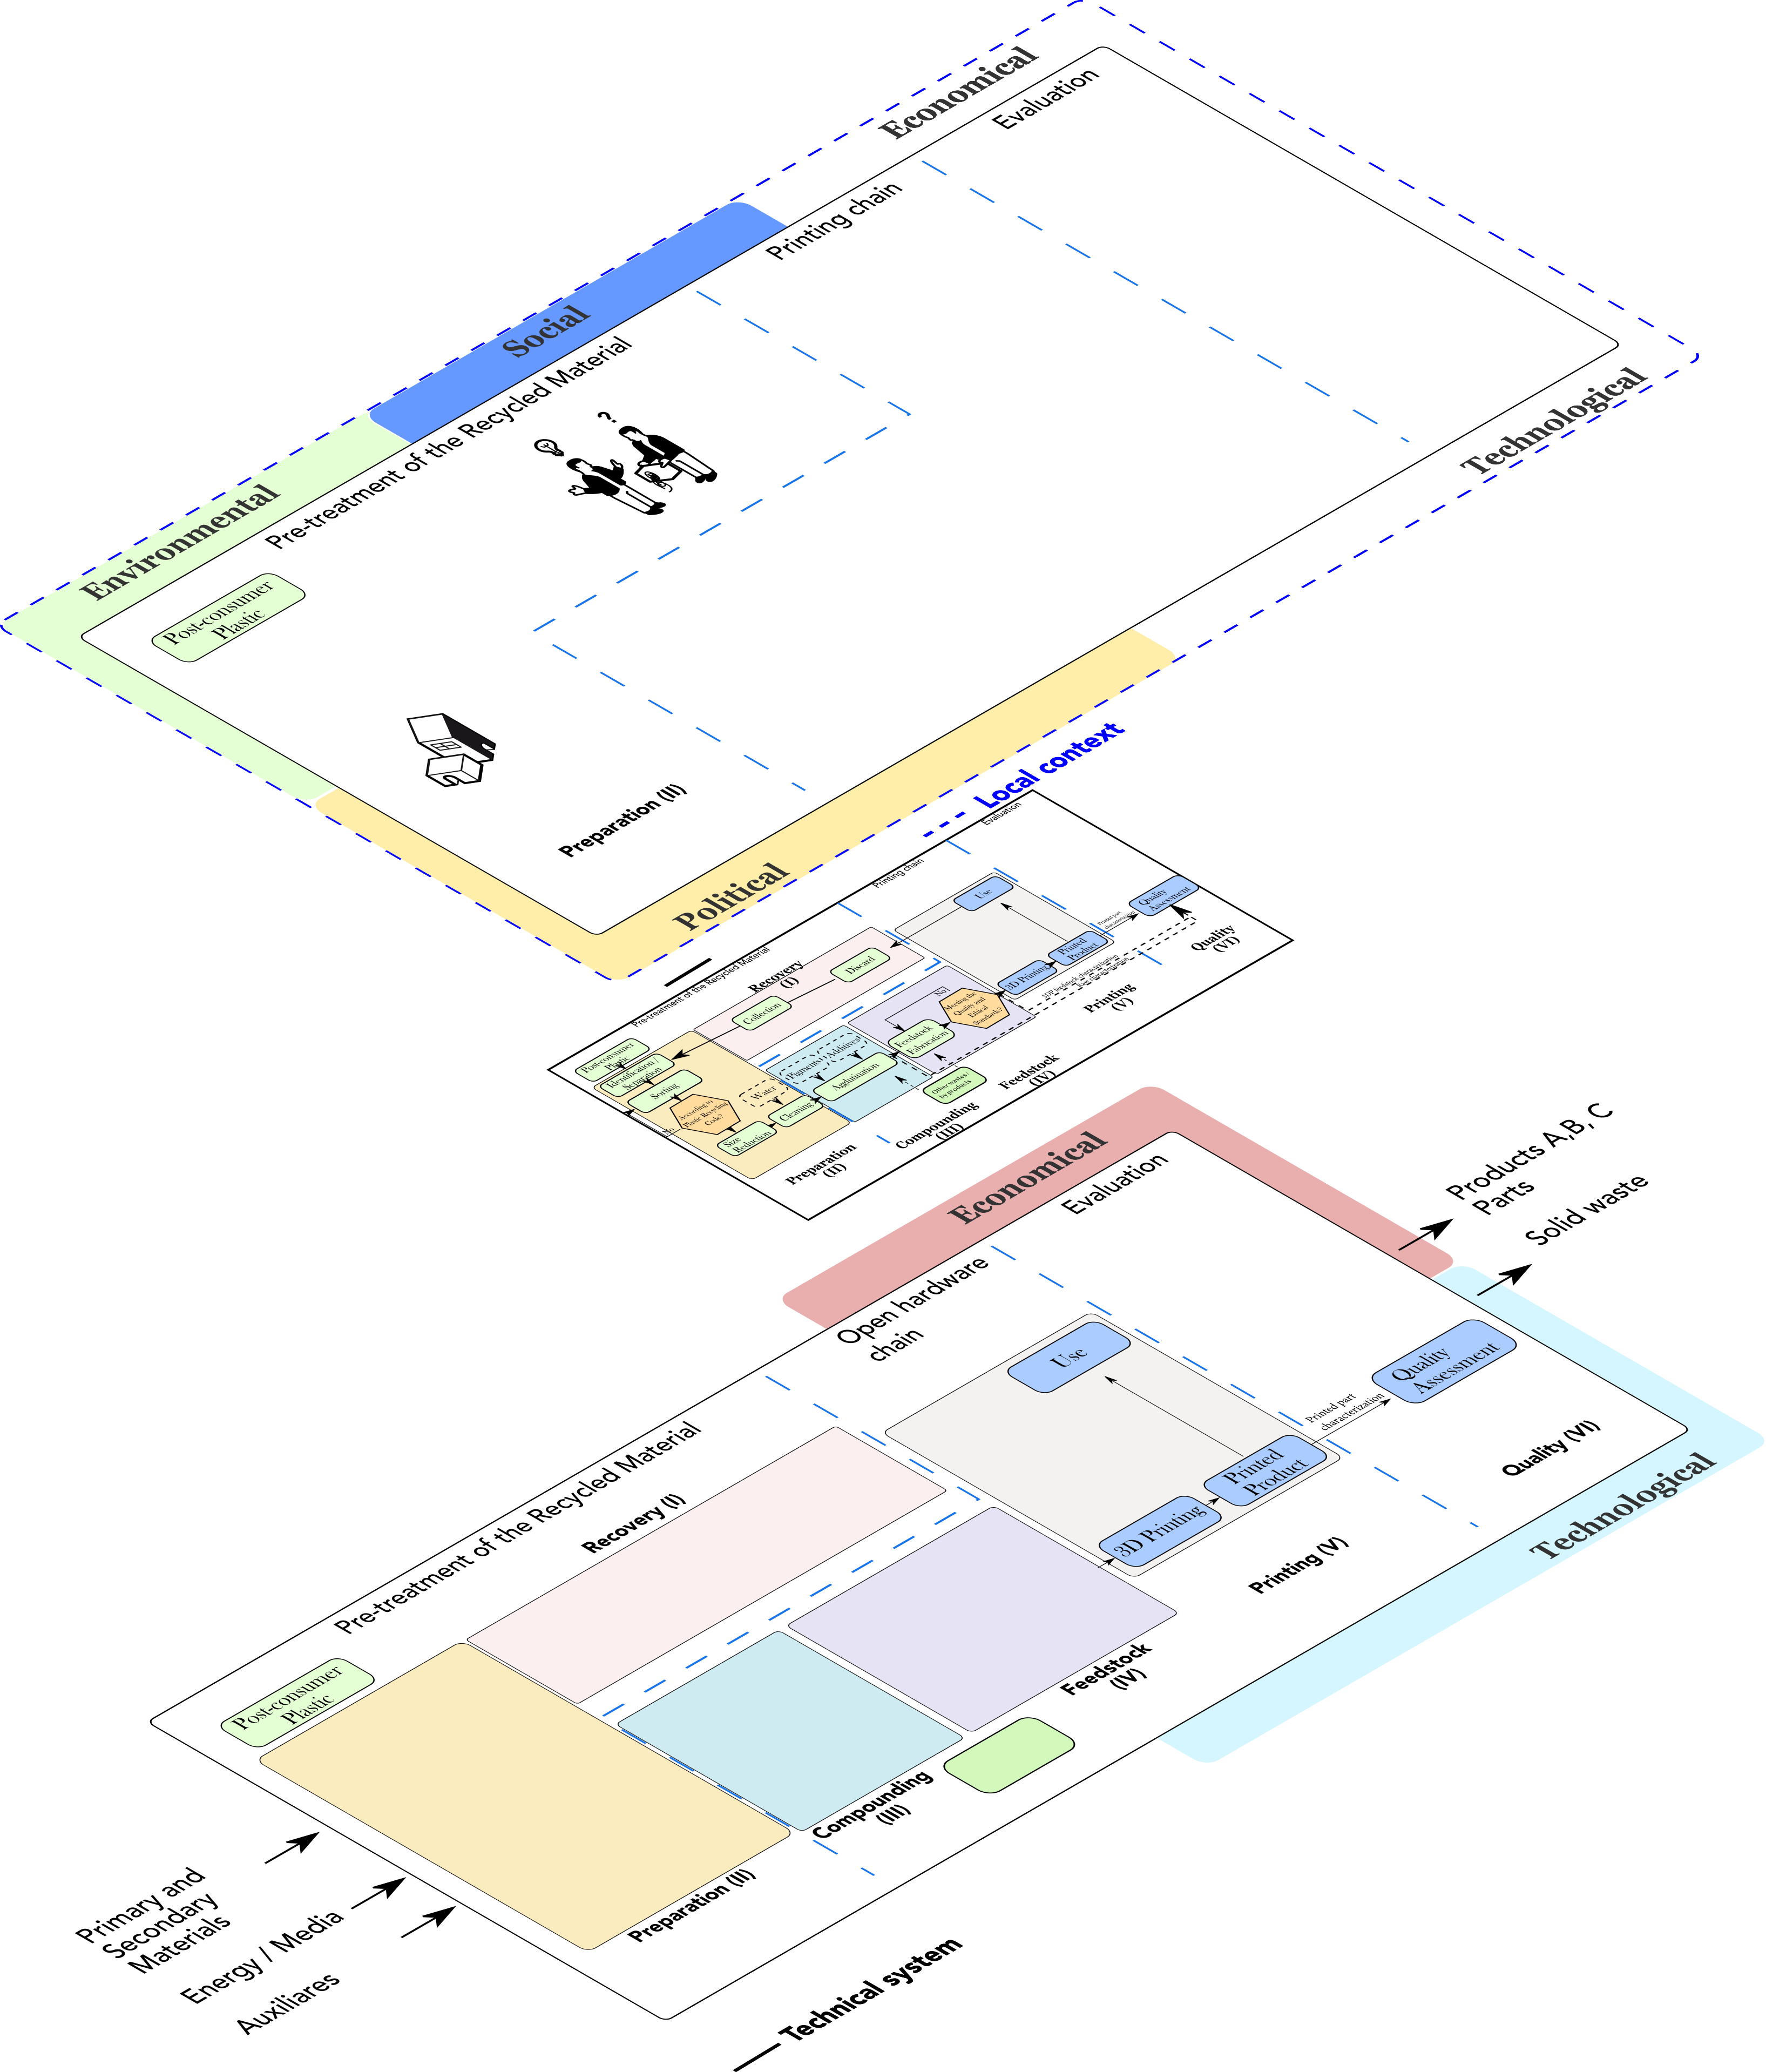
\includegraphics[width=\linewidth]{Figures/Levels.png}
    \caption{Methodology}
    \label{fig:levels}
\end{wrapfigure}

Therefore, the main objective of this project is \textbf{to establish a
systemic methodological blueprint to fully understand how to design,
implement and (e)valuate urban production systems based on the
\emph{``Design Global / Manufacturing local''} principles }. The
deployment of circularity marks a return to a more productive design of
the city, that must consider the natural and urban ecosystem services,
the strengthened of the resilience capacities and taking into account
the energy sobriety of european territories. Thus, this project seeks
two level targets:

\begin{enumerate}
\def\labelenumi{\arabic{enumi})}
\tightlist
\item
  The scientific understanding of the design of socio-technical
  configurations of urban production systems based on distributed
  plastic recycling as resilience strategy.\\
\item
  Holistic and pluralistic (e)valuation of the open source appropriate
  technologies and design as assets for urban territorial development.
\end{enumerate}

I aims further develop the distributed recycling analysing the as
illustrated in figure \ref{fig:levels} (1) technical layer (2) urban
layer (3) Evaluation layer.

Based on that, table XX presents an outline of the research question of
the three major layers to consider in this project.

\small

\begin{longtable}[]{@{}
  >{\raggedright\arraybackslash}p{(\columnwidth - 0\tabcolsep) * \real{1.0000}}@{}}
\toprule()
\begin{minipage}[b]{\linewidth}\raggedright
\textbf{Challenge 1: Urban systems' role in the deployment of the
circularity.}
\end{minipage} \\
\midrule()
\endhead
\begin{minipage}[t]{\linewidth}\raggedright
In order to identify the design process of an urban circular production
system, some relevant questions are the following:

\begin{itemize}
\item
  How to dimension production systems to be consistent with the
  resources and materials (recycled plastics) (first and second hand)
  considered as local ?
\item
  How to establish the link to integrate territorial planning priorities
  with respect to production systems priorities within an urban circular
  economy context?
\item
  What are the acceptability conditions for the deployment of urban
  demostrators of circularity?
\item
  How to identify the opportunities and barriers from a social,
  technological, political and legal point of view for the
  implementation of an urban production/recycling network?
\item
  What strategies can be implemented so that socio-technical systems of
  circular production can be in line with urban needs and their
  contribution to the SDGs?
\item
  How to establish an open source value chain in order to foster
  resilience and technological and energetic sobriety of the urban
  territory?
\item
  How would the implementation of urban production systems affect the
  functional blocks of an urban territory?
\end{itemize}
\end{minipage} \\
\bottomrule()
\end{longtable}

\begin{longtable}[]{@{}
  >{\raggedright\arraybackslash}p{(\columnwidth - 0\tabcolsep) * \real{1.0000}}@{}}
\toprule()
\begin{minipage}[b]{\linewidth}\raggedright
\textbf{Challenge 2: Systematize the open source technodiversity as
territorial asset.}
\end{minipage} \\
\midrule()
\endhead
\begin{minipage}[t]{\linewidth}\raggedright
To implement an open source appropriate technology ecosystem suitable
for circular urban production system, some relevant research questions
are the following:

\begin{itemize}
\item
  How to design a technodiversity baseline based on open source
  appropriate technologies (OSAT) for distributed recycling?
\item
  How can the design process of an appropriate open source technology be
  analyzed to avoid what is known as the Jevons paradox?
\item
  How to facilitate the adoption of open source practices and tools, for
  a public that goes beyond the fablab/makerspaces that have been
  pioneers?
\item
  What would be the relevant business model for open hardware adoption
  to allow the introduction of open source tools and practices?
\item
  How to evaluate the degree of maturity of a small company so that
  within its strategy it can implement the adoption of open hardware as
  a disruptive practice?
\item
  What open source technologies needed to develop and implement a urban
  closed-loop suply chain ?
\item
  How open source technologies would allow the development of urban
  productive systems in coherence to favor the resilience of the
  territory?
\item
  What are the core competences needed in an open source ecosystem for
  urban circularity?
\end{itemize}
\end{minipage} \\
\bottomrule()
\end{longtable}

\begin{longtable}[]{@{}
  >{\raggedright\arraybackslash}p{(\columnwidth - 0\tabcolsep) * \real{1.0000}}@{}}
\toprule()
\begin{minipage}[b]{\linewidth}\raggedright
\textbf{Challenge 3: Pluralistic (e)valuation of distributed recycling
systems.}
\end{minipage} \\
\midrule()
\endhead
\begin{minipage}[t]{\linewidth}\raggedright
In order to (e)valuate in a pluralistic way the development and
implementation of urban distributed units, some relevant questions are
the following:

\begin{itemize}
\item
  How to connect ecological and economic indicators within the same
  evaluation framework?
\item
  Which territorial and production system indicators would make it
  possible to establish a minimum scale of operation, but also a maximum
  scale that respects urban ecosystem services?
\item
  How to establish scenarios of evolution and impact so that territorial
  decision-makers can encourage the adoption and piloting of these
  initiatives?
\item
  What would be the relevant functional unit to delimit the range of
  action of the production/recycling system within the urban metabolism?
\item
  What are the necessary considerations to represent the preferences of
  the stakeholders in the decision-making process of integration urban /
  manufacturing systems?
\item
  How to support the process form collective consensus to the deployment
  of these emerging systems under a purpose oriented approach?
\end{itemize}
\end{minipage} \\
\bottomrule()
\end{longtable}

\normalsize

\hypertarget{an-impact-project}{%
\subsection{3. An Impact project}\label{an-impact-project}}

\begin{itemize}
\item
  \textbf{Main scientific impacts.} This project aims to make a the
  breakthrough understating of the implementation and evaluation of the
  distri design of sustainability of distributed urban recycling systems
\item
  \textbf{Main societal impacts.} If the expected modeling are
  confirmed, the outcome of this pproject will allow urban and technical
  desicion-makers the implementation of local recycling circuits of
  available plastic waste by means of small, ro distribed recycling
  socio-technical units.
\end{itemize}

\hypertarget{section-b.-methodology}{%
\section{Section b. Methodology}\label{section-b.-methodology}}

\hypertarget{introduction-the-scientific-methodology}{%
\subsection{3. Introduction the scientific
methodology}\label{introduction-the-scientific-methodology}}

\begin{wrapfigure}[13]{r}[0pt]{0.35\textwidth}
\centering
    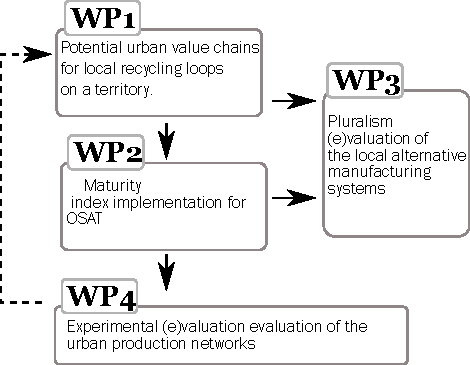
\includegraphics[width=\linewidth]{Figures/WPs.pdf}
    \caption{Methodology}
    \label{fig:WPs}
\end{wrapfigure}

This project implements a methodology made of four working packages
(WP), as illustrated in Fig. \ref{fig:WPs}. We recognize appropriate
intermediate objectives (Tasks) and we individuate the specific
interventions of the members of the research team. Moreover, we discuss
the particular methodologies that we plan to adopt and we make a balance
among the risks and gains associated to each action. The aim of WP1 is
to set a baseline for an integrative and critical analysis of urban
territory in the frame of micro-value chains for manufacturing/recycling
production. This working package gives the insights for the WP2, and
WP3, which are key of the project. The WP2 seeks to consolidate
systematize a design process for OSAT for a complete distributed
manufacturing/recycling process establishing an unit maturity level
index, but more important, a system maturity level for the integration
into an urban ecosystem. The main output is to establish a complete OSAT
design framework ecosystems to valorize the waste niches opportunities
identified in WP1. The WP3 aims to identify a pluralistic (e)valuation
framework for the urban closed-loop system network integrating three
essential issues: sustainability, resiliency, and agility into a
circular economy praxis. Finally, WP4 is dedicated to the
experimentation of the several case studies of the urban circular
manufacturing taking as exemple into at case studies the implementation
of the Green Fablab Project at the third place of OK3 at Nancy-France.
The object is to replicate this analysis in other territories such
Chile, in collaboration with Prof.~Pavlo Santander at the university of
Santiago de Chile, and in Canada with collaboration of Prof.~Joshua
Pearce at Western University. Work packages are synthetically detailed
hereinafter. Work packages are synthetically detailed hereinafter.

\hypertarget{wp-1-theoretical-baseline-on-urban-value-chains}{%
\subsubsection{WP 1: Theoretical baseline on urban value
chains}\label{wp-1-theoretical-baseline-on-urban-value-chains}}

\textbf{Main objective}: This WP deals with the development of the
needed aid-decision tools to unfold the potentials micro-value chains
and exchange flows induced by distributed recycling. This framework is
based on the urban spatial analysis and stakeholders characteristics as
an entry point. In this work package, the major output will be an
aid-decision tool to possible be the input for WP2 and WP3. The steps
that I will follow to develop aid-decision tool used in this project.

\hypertarget{task-1.1-to-establish-a-methodological-framework-that-close-the-existing-data-gaps-in-terms-of-secondary-plastic-material-availability-at-the-urban-level-considering-its-complexity-level-of-revalorization.}{%
\paragraph{Task 1.1: to establish a methodological framework that close
the existing data gaps in terms of secondary plastic material
availability at the urban level considering its complexity level of
revalorization.}\label{task-1.1-to-establish-a-methodological-framework-that-close-the-existing-data-gaps-in-terms-of-secondary-plastic-material-availability-at-the-urban-level-considering-its-complexity-level-of-revalorization.}}

The monitoring and assessing material consumption and material
productivity is critical, both from a macroeconomic perspective ---to
assess whether sufficient action has been taken, as well as from a local
perspective--- to support local decision makers in setting new
priorities toward long-term
objectives\textsuperscript{\protect\hyperlink{ref-Bianchi2020}{117}}.
The goal is to define a \emph{\{territory x material\}} index from a
quantitative approach and urban metabolism to study resource use in a
urban city. This assessment aims to quantify hotspots (availability and
level of contamination) based on territorial and footprint indicators
and assess scenarios for the design of a recycling closed-loop supply
chain. For the case of plastic material, this is particularly relevant
given ambitious circularity targets that certain governments have
putting in
place\textsuperscript{\protect\hyperlink{ref-france}{\textbf{france?}}}
due to the their impact. The priority is to reveal a list of `suitable'
secondary materials wastes at the urban level that today are not fully
understood and valorized. This analysis will be carried out at least
every year, and if possible more frequently to see if there is a change
or seasonality in the composition of this untreated waste.

\hypertarget{task-1.2-qualitative-analysis-of-the-established-valorization-systems-of-recycling-the-urban-territorial-priorities-and-stakeholders-in-the-frame-of-ecosystems-services.}{%
\paragraph{Task 1.2: Qualitative analysis of the established
valorization systems of recycling the urban territorial priorities and
stakeholders in the frame of ecosystems
services.}\label{task-1.2-qualitative-analysis-of-the-established-valorization-systems-of-recycling-the-urban-territorial-priorities-and-stakeholders-in-the-frame-of-ecosystems-services.}}

The main aim in this task is a methodological tool to align priorities
in the development of urban production and urban development priorities,
and in that way, to take informed decisions on the development of urban
(circular) factories in a local territory.

\hypertarget{task-1.3-multi-criteria-analysis-of-the-urban-territorial-priorities-and-stakeholders-in-the-frame-of-ecosystems-services.}{%
\paragraph{Task 1.3: Multi-criteria analysis of the urban territorial
priorities and stakeholders in the frame of ecosystems
services.}\label{task-1.3-multi-criteria-analysis-of-the-urban-territorial-priorities-and-stakeholders-in-the-frame-of-ecosystems-services.}}

The main aim in this task is a methodological tool to align priorities
in the development of urban production and urban development priorities,
and in that way, to take informed decisions on the development of urban
(circular) factories in a local territory.

Human life and activities rely on ecosystem services (ES) provided by
nature. The ecosystem services are the ecological characteristics,
functions or processes that contribute (actively or passively) to the
human
well-being\textsuperscript{\protect\hyperlink{ref-Costanza1997}{118},\protect\hyperlink{ref-Costanza2017}{119}}.
Ecosystem goods (e.g; Food) and services (e.g.~waste assimilation)
illustrate the benefits that human derive from the ecosystem
functions\textsuperscript{\protect\hyperlink{ref-Costanza1997}{118}}.
The ecosystem services do not flow to human well-being without crucial
interactions with the different forms of capital (Natural, Social,
Human, Built), which entails the need of understanding, modelling,
measuring, and managing ES in a transdisciplinary approach. Likewise,
the concept of ecosystem dis-service denotes the processes and functions
that affect humans in `negative' way, making damage and
costs\textsuperscript{\protect\hyperlink{ref-ref}{\textbf{ref?}}}. With
the concentration of people and activities in cities, these services are
intensively utilized in urban space to an extent that in most cases
cannot be provided by the local ecosystem. Thus, cities (and urban
factories) have to rely on supply regions and connection to their
hinterland. One major point that ES make clear is to raise awareness on
the recognition of interdependence of human, humanity's primary
dependances on the `functions of' natural capital which reflects the
fact that, however they may perceive themselves, humans are part of, and
not apart from,
nature\textsuperscript{\protect\hyperlink{ref-Ekins2003}{120}}. This
entails the necessity to create knowledge for transdisciplinary
approaches using ES as boundary object for sustainability for diverse
stakeholders\textsuperscript{\protect\hyperlink{ref-Honeck2021}{121}}.

As starting point, we will analyze the sites and the territories
concerned by the Green Fablab project, namely the urban community of
``Grand Nancy'' (CUGN). We benefit from the support of the municipality
and the recognition of the project in the local area. We will be able to
perform a field diagnosis of this territory to map and characterize the
existing stakeholders needs, a SWOT analysis (Strengths, Weaknesses,
Opportunities, and Threats) including technical, economic and
environmental evaluations of the existing value chains, to understand
where the value chain could be positioned in the future. This test is
the first step to possible replicate the analysis for other terrotories.

\small

\normalsize

\hypertarget{wp-2-maturity-and-technodiverstity-level-of-the-open-source-appropriate-technology-for-the-degrowth-paradigm}{%
\subsubsection{WP 2: Maturity and technodiverstity level of the open
source appropriate technology for the degrowth
paradigm}\label{wp-2-maturity-and-technodiverstity-level-of-the-open-source-appropriate-technology-for-the-degrowth-paradigm}}

\textbf{Main objective}: The WP2 will be focused on the unit- and
facility-level to better understand how the design process of open
source appropriate technology can be implemented in urban
micro-recycling systems. Nevertheless, a future establishment of
technical standards bringing clarity in this emerging and moving field
is needed.

The main purpose of this task is to leverage a resilient
manufacturing\textsuperscript{\protect\hyperlink{ref-xu2021e}{116},\protect\hyperlink{ref-zhang2011}{122}}
under the logic of Design Global/Manufacture Local robustness.\\
To do so, three major tasks are seen:

\hypertarget{design-design-of-open-source}{%
\paragraph{(2.1) Design design of Open
Source}\label{design-design-of-open-source}}

definition of a scientific literature and critical analysis on the
adoption and barriers of the open source appropriate technologies with
particular focus on distributed recycling considering the modularity

The definition of a scientific literature and critical analysis on the
adoption\textsuperscript{\protect\hyperlink{ref-reinauer2021}{123}} and
barriers of the open-source appropriate technologies with particular
focus on distributed recycling considering the modularity
types\textsuperscript{\protect\hyperlink{ref-gavras2021}{124}}, gaps in
the hardware development and .

\hypertarget{mapping-of-newadapted-practices-and-tools-that-would-be-needed-to-support-local-manufacturers-and-local-decision-makers-to-navigate-and-overcome-the-challenges-of-distributed-recycling.}{%
\paragraph{(2.2) Mapping of new/adapted practices and tools that would
be needed to support local manufacturers and local decision makers to
navigate and overcome the challenges of distributed
recycling.}\label{mapping-of-newadapted-practices-and-tools-that-would-be-needed-to-support-local-manufacturers-and-local-decision-makers-to-navigate-and-overcome-the-challenges-of-distributed-recycling.}}

\hypertarget{identification-a-system-maturity-level-that-enable-the-constitution-of-urban-closed-loop-supply-chain-.}{%
\paragraph{(2.3) Identification a system maturity level that enable the
constitution of urban closed-loop supply chain
.}\label{identification-a-system-maturity-level-that-enable-the-constitution-of-urban-closed-loop-supply-chain-.}}

\hypertarget{wp-3-pluralistic-evaluation-of-distributed-recycling-systems}{%
\subsubsection{WP 3: Pluralistic (e)valuation of distributed recycling
systems}\label{wp-3-pluralistic-evaluation-of-distributed-recycling-systems}}

In parallel of WP2, the WP3 aims to consolidate aid-decision tool to
reveal and better understand under which conditions these distributed
recycling/manufacturing urban chains are pertinent for the local
territory. This tool describe and characterize the new value chain to
include new form of pluralism
valuation\textsuperscript{\protect\hyperlink{ref-gunton2022}{125}} and
techno-ecological
interactions\textsuperscript{\protect\hyperlink{ref-Saladini2018}{115},\protect\hyperlink{ref-Liu2020c}{126},\protect\hyperlink{ref-Liu2019g}{127}}.
More important to avoid Jevons
paradox\textsuperscript{\protect\hyperlink{ref-giampietro2018}{128}}, it
is determine the scale of action considering the technical maturity,
economic viability and environmental respect of the ecosystem services.
In (4.1), one strategical point in sustainability relies on explicitly
account for their demand and supply of of ecosystem goods and services
framework given by the micro-value
chains\textsuperscript{\protect\hyperlink{ref-Diwekar2021}{129}}. then
(4.2), the main aim is to reveal the components and the structure of the
urban circular networks to the combining Material Flow
Analysis\textsuperscript{\protect\hyperlink{ref-saidani2021}{130}},
System
Dynamics\textsuperscript{\protect\hyperlink{ref-kuo2021}{131}--\protect\hyperlink{ref-perez-perez2021}{135}}
and Circularity
Indicators\textsuperscript{\protect\hyperlink{ref-saidani2019}{136}}.

\hypertarget{wp-4-experimentation-and-deployment-in-function-of-the-local-territory}{%
\subsubsection{WP 4: Experimentation and deployment in function of the
local
territory}\label{wp-4-experimentation-and-deployment-in-function-of-the-local-territory}}

The WP4 aims to consolidate a starting point for a longitudinal
study\textsuperscript{\protect\hyperlink{ref-langley2013}{137}} to
evaluate of the implementation these distributed recycling strategies at
a urban territorial level. WP4 is devoted to the iteration and
evaluation of the urban production networks to deep understand the
evolution. 4.1) Several case studies of distributed fabrication /
recycling will be documented and developed in complement with a
comparative and contextualized Life Cycle Assessment (LCA) of the new
secondary AM material compared to actual materials. 4.2) A strategic
roadmap will be a major delivered to understand the possible evolution
of

To pass from ecodesign to an operation design for sustainability
approach, this WP4 will be based ten different models at operational,
tactical, and strategical
levels\textsuperscript{\protect\hyperlink{ref-SousaRocha2019}{138}}.

\hypertarget{conceptual-risk-and-fesability-assessment}{%
\subsection{3. Conceptual risk and fesability
assessment}\label{conceptual-risk-and-fesability-assessment}}

SDRAM is a high operation and conceptual-risk project mainly because the
integration of multiples disciplines in a one basis framework need to
establish boundary object to have a coherent framework.

\small

\begin{longtable}[]{@{}
  >{\raggedright\arraybackslash}p{(\columnwidth - 10\tabcolsep) * \real{0.0233}}
  >{\raggedright\arraybackslash}p{(\columnwidth - 10\tabcolsep) * \real{0.2744}}
  >{\raggedright\arraybackslash}p{(\columnwidth - 10\tabcolsep) * \real{0.1256}}
  >{\raggedright\arraybackslash}p{(\columnwidth - 10\tabcolsep) * \real{0.0977}}
  >{\raggedright\arraybackslash}p{(\columnwidth - 10\tabcolsep) * \real{0.0419}}
  >{\raggedright\arraybackslash}p{(\columnwidth - 10\tabcolsep) * \real{0.4372}}@{}}
\caption{ss}\tabularnewline
\toprule()
\begin{minipage}[b]{\linewidth}\raggedright
ID
\end{minipage} & \begin{minipage}[b]{\linewidth}\raggedright
Risk items
\end{minipage} & \begin{minipage}[b]{\linewidth}\raggedright
Effect of the risk
\end{minipage} & \begin{minipage}[b]{\linewidth}\raggedright
Causes of the risk
\end{minipage} & \begin{minipage}[b]{\linewidth}\raggedright
Grade
\end{minipage} & \begin{minipage}[b]{\linewidth}\raggedright
Actions to minimize the risk
\end{minipage} \\
\midrule()
\endfirsthead
\toprule()
\begin{minipage}[b]{\linewidth}\raggedright
ID
\end{minipage} & \begin{minipage}[b]{\linewidth}\raggedright
Risk items
\end{minipage} & \begin{minipage}[b]{\linewidth}\raggedright
Effect of the risk
\end{minipage} & \begin{minipage}[b]{\linewidth}\raggedright
Causes of the risk
\end{minipage} & \begin{minipage}[b]{\linewidth}\raggedright
Grade
\end{minipage} & \begin{minipage}[b]{\linewidth}\raggedright
Actions to minimize the risk
\end{minipage} \\
\midrule()
\endhead
1 & Difficulty to data access to local territorial diagnosis &
Constraint to define WP1 & & Middle & There have been pre-exists between
the partners and these territories and recycling actors. \\
2 & & & & & \\
3 & & & & & \\
\bottomrule()
\end{longtable}

\begin{longtable}[]{@{}
  >{\raggedright\arraybackslash}p{(\columnwidth - 4\tabcolsep) * \real{0.0485}}
  >{\raggedright\arraybackslash}p{(\columnwidth - 4\tabcolsep) * \real{0.8252}}
  >{\raggedright\arraybackslash}p{(\columnwidth - 4\tabcolsep) * \real{0.1262}}@{}}
\caption{Feasible challengues in the methodology}\tabularnewline
\toprule()
\begin{minipage}[b]{\linewidth}\raggedright
ID
\end{minipage} & \begin{minipage}[b]{\linewidth}\raggedright
Main challengues
\end{minipage} & \begin{minipage}[b]{\linewidth}\raggedright
Feasibility
\end{minipage} \\
\midrule()
\endfirsthead
\toprule()
\begin{minipage}[b]{\linewidth}\raggedright
ID
\end{minipage} & \begin{minipage}[b]{\linewidth}\raggedright
Main challengues
\end{minipage} & \begin{minipage}[b]{\linewidth}\raggedright
Feasibility
\end{minipage} \\
\midrule()
\endhead
1 & Theoretical baseline on urban value chains & \\
2 & Maturity level and technodiverstity level of the open source
appropritte technology & \\
3 & Pluralism (e)valuation of the distributed recycling systems & \\
4 & & \\
\bottomrule()
\end{longtable}

\normalsize

\hypertarget{resources-and-budget}{%
\subsection{5. Resources and budget}\label{resources-and-budget}}

\hypertarget{the-research-team}{%
\subsubsection{The research team}\label{the-research-team}}

\begin{wrapfigure}{r}[0pt]{0.6\textwidth}
\centering
    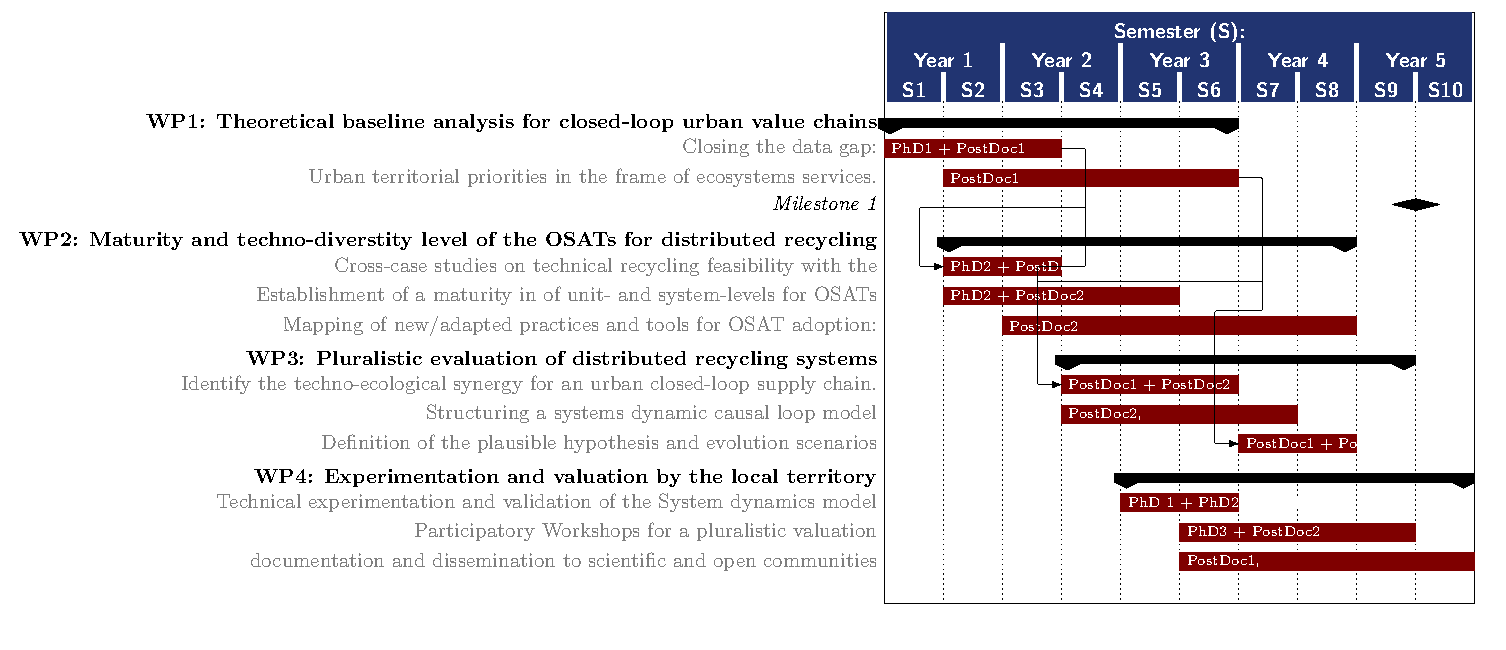
\includegraphics[width=0.9\linewidth]{Gantt/Gantt-B1.pdf}
    \caption{Gantt diagram and task allocation}
    \label{fig:gantt-b1}
\end{wrapfigure}

The budget required for the development of SDRAM is XXX €. The most
significant cost is the personnel cost (XXXX € - XX \%). Minor cost
cover the purchase of open hardware equipement (XXXX € - XX \%), travels
for dissemination of results (XXXX € - XX \%), Open access fees for at
least 8 publications (XXXX € - XX \%). \%

As for me, I will dedicate 42 p.m. of my work to manage this five-year
exciting project. I will manage each phase of the project, in the full
awareness of the responsibility that I will have in its successful
realization, which highly depends on my capability to -humanely and
scientifically- conduct, coordinate and supervise the activities carried
on by the scientific team.

\newpage

\hypertarget{references}{%
\subsection*{References}\label{references}}
\addcontentsline{toc}{subsection}{References}

\hypertarget{refs}{}
\begin{CSLReferences}{0}{0}
\leavevmode\vadjust pre{\hypertarget{ref-kanger2022}{}}%
\CSLLeftMargin{1. }%
\CSLRightInline{Kanger L, Bone F, Rotolo D, et al.
\href{https://doi.org/10.1016/j.techfore.2022.121491}{Deep transitions:
{A} mixed methods study of the historical evolution of mass production}.
\emph{Technological Forecasting and Social Change} 2022; 177: 121491.}

\leavevmode\vadjust pre{\hypertarget{ref-raworth2017}{}}%
\CSLLeftMargin{2. }%
\CSLRightInline{Raworth K.
\href{https://doi.org/10.1016/S2542-5196(17)30028-1}{A {Doughnut} for
the {Anthropocene}: Humanity's compass in the 21st century}. \emph{The
Lancet Planetary Health} 2017; 1: e48--e49.}

\leavevmode\vadjust pre{\hypertarget{ref-steffen2018}{}}%
\CSLLeftMargin{3. }%
\CSLRightInline{Steffen W, Rockström J, Richardson K, et al.
\href{https://doi.org/10.1073/pnas.1810141115}{Trajectories of the
{Earth System} in the {Anthropocene}}. \emph{Proceedings of the National
Academy of Sciences} 2018; 115: 8252--8259.}

\leavevmode\vadjust pre{\hypertarget{ref-steffen2011}{}}%
\CSLLeftMargin{4. }%
\CSLRightInline{Steffen W, Grinevald J, Crutzen P, et al.
\href{https://doi.org/10.1098/rsta.2010.0327}{The {Anthropocene}:
Conceptual and historical perspectives}. \emph{Philosophical
Transactions of the Royal Society A: Mathematical, Physical and
Engineering Sciences} 2011; 369: 842--867.}

\leavevmode\vadjust pre{\hypertarget{ref-porta2021}{}}%
\CSLLeftMargin{5. }%
\CSLRightInline{Porta R.
\href{https://doi.org/10.1002/2211-5463.13122}{Anthropocene, the plastic
age and future perspectives}. \emph{FEBS Open Bio} 2021; 11: 948--953.}

\leavevmode\vadjust pre{\hypertarget{ref-de-la-torre2021}{}}%
\CSLLeftMargin{6. }%
\CSLRightInline{De-la-Torre GE, Dioses-Salinas DC, Pizarro-Ortega CI, et
al. \href{https://doi.org/10.1016/j.scitotenv.2020.142216}{New plastic
formations in the {Anthropocene}}. \emph{Science of The Total
Environment} 2021; 754: 142216.}

\leavevmode\vadjust pre{\hypertarget{ref-ONeill2018}{}}%
\CSLLeftMargin{7. }%
\CSLRightInline{O'Neill DW, Fanning AL, Lamb WF, et al.
\href{https://doi.org/10.1038/s41893-018-0021-4}{A good life for all
within planetary boundaries}. \emph{Nature Sustainability} 2018; 1:
88--95.}

\leavevmode\vadjust pre{\hypertarget{ref-Rockstrom2009}{}}%
\CSLLeftMargin{8. }%
\CSLRightInline{Rockström J, Steffen W, Noone K, et al.
\href{https://doi.org/10.1038/461472a}{A safe operating space for
humanity}. \emph{Nature} 2009; 461: 472--475.}

\leavevmode\vadjust pre{\hypertarget{ref-Iles2013}{}}%
\CSLLeftMargin{9. }%
\CSLRightInline{Iles A, Martin AN.
\href{https://doi.org/10.1016/j.jclepro.2012.05.008}{Expanding
bioplastics production: Sustainable business innovation in the chemical
industry}. \emph{Journal of Cleaner Production} 2013; 45: 38--49.}

\leavevmode\vadjust pre{\hypertarget{ref-DeVargasMores2018}{}}%
\CSLLeftMargin{10. }%
\CSLRightInline{de Vargas Mores G, Finocchio CPS, Barichello R, et al.
\href{https://doi.org/10.1016/j.jclepro.2017.12.138}{Sustainability and
innovation in the {Brazilian} supply chain of green plastic}.
\emph{Journal of Cleaner Production} 2018; 177: 12--18.}

\leavevmode\vadjust pre{\hypertarget{ref-Paletta2019}{}}%
\CSLLeftMargin{11. }%
\CSLRightInline{Paletta A, Leal Filho W, Balogun AL, et al.
\href{https://doi.org/10.1016/j.jclepro.2019.118149}{Barriers and
challenges to plastics valorisation in the context of a circular
economy: {Case} studies from {Italy}}. \emph{Journal of Cleaner
Production} 2019; 241: 118149.}

\leavevmode\vadjust pre{\hypertarget{ref-Gong2020}{}}%
\CSLLeftMargin{12. }%
\CSLRightInline{Gong Y, Putnam E, You W, et al.
\href{https://doi.org/10.1016/j.jclepro.2019.118941}{Investigation into
circular economy of plastics: {The} case of the {UK} fast moving
consumer goods industry}. \emph{Journal of Cleaner Production} 2020;
244: 118941.}

\leavevmode\vadjust pre{\hypertarget{ref-Ma2020}{}}%
\CSLLeftMargin{13. }%
\CSLRightInline{Ma X, Park C, Moultrie J.
\href{https://doi.org/10.1016/j.jclepro.2020.120492}{Factors for
eliminating plastic in packaging: {The European FMCG} experts' view}.
\emph{Journal of Cleaner Production} 2020; 256: 120492.}

\leavevmode\vadjust pre{\hypertarget{ref-Confente2020}{}}%
\CSLLeftMargin{14. }%
\CSLRightInline{Confente I, Scarpi D, Russo I.
\href{https://doi.org/10.1016/j.jbusres.2019.10.030}{Marketing a new
generation of bio-plastics products for a circular economy: {The} role
of green self-identity, self-congruity, and perceived value}.
\emph{Journal of Business Research} 2020; 112: 431--439.}

\leavevmode\vadjust pre{\hypertarget{ref-Friedrich2020}{}}%
\CSLLeftMargin{15. }%
\CSLRightInline{Friedrich D.
\href{https://doi.org/10.1016/j.jclepro.2020.121128}{How regulatory
measures towards biobased packaging influence the strategic behaviour of
the retail industry: {A} microempirical study}. \emph{Journal of Cleaner
Production} 2020; 260: 121128.}

\leavevmode\vadjust pre{\hypertarget{ref-Filho2021}{}}%
\CSLLeftMargin{16. }%
\CSLRightInline{Filho WL, Salvia AL, Bonoli A, et al.
\href{https://doi.org/10.1016/j.scitotenv.2020.142732}{An assessment of
attitudes towards plastics and bioplastics in {Europe}}. \emph{Science
of The Total Environment} 2021; 755: 142732.}

\leavevmode\vadjust pre{\hypertarget{ref-Huysveld2019}{}}%
\CSLLeftMargin{17. }%
\CSLRightInline{Huysveld S, Hubo S, Ragaert K, et al.
\href{https://doi.org/10.1016/j.jclepro.2018.11.110}{Advancing circular
economy benefit indicators and application on open-loop recycling of
mixed and contaminated plastic waste fractions}. \emph{Journal of
Cleaner Production} 2019; 211: 1--13.}

\leavevmode\vadjust pre{\hypertarget{ref-Pazienza2020}{}}%
\CSLLeftMargin{18. }%
\CSLRightInline{Pazienza P, De Lucia C.
\href{https://doi.org/10.1002/bse.2445}{The {EU} policy for a plastic
economy: {Reflections} on a sectoral implementation strategy}.
\emph{Business Strategy and the Environment} 2020; 29: 779--788.}

\leavevmode\vadjust pre{\hypertarget{ref-zhen2021}{}}%
\CSLLeftMargin{19. }%
\CSLRightInline{Zhen H, Gao W, Yuan K, et al.
\href{https://doi.org/10.1016/j.ecoser.2021.101323}{Internalizing
externalities through net ecosystem service analysis\textendash{{A}}
case study of greenhouse vegetable farms in {Beijing}}. \emph{Ecosystem
Services} 2021; 50: 101323.}

\leavevmode\vadjust pre{\hypertarget{ref-Murray2017}{}}%
\CSLLeftMargin{20. }%
\CSLRightInline{Murray A, Skene K, Haynes K.
\href{https://doi.org/10.1007/s10551-015-2693-2}{The {Circular Economy}:
{An Interdisciplinary Exploration} of the {Concept} and {Application} in
a {Global Context}}. \emph{Journal of Business Ethics} 2017; 140:
369--380.}

\leavevmode\vadjust pre{\hypertarget{ref-EC2015}{}}%
\CSLLeftMargin{21. }%
\CSLRightInline{European Commision.
\href{https://doi.org/10.1017/CBO9781107415324.004}{Summary for
{Policymakers}}. In: Intergovernmental Panel on Climate Change (ed)
\emph{Climate {Change} 2013 - {The Physical Science Basis}}.
{Cambridge}: {Cambridge University Press}, pp. 1--30.}

\leavevmode\vadjust pre{\hypertarget{ref-EllenMacArthurFoundation2015}{}}%
\CSLLeftMargin{22. }%
\CSLRightInline{Ellen MacArthur Foundation.
\href{https://doi.org/Article}{Growth within: A circular economy vision
for a competitive europe}. \emph{Ellen MacArthur Foundation} 2015; 100.}

\leavevmode\vadjust pre{\hypertarget{ref-nobre2021}{}}%
\CSLLeftMargin{23. }%
\CSLRightInline{Nobre GC, Tavares E.
\href{https://doi.org/10.1016/j.jclepro.2021.127973}{The quest for a
circular economy final definition: {A} scientific perspective}.
\emph{Journal of Cleaner Production} 2021; 314: 127973.}

\leavevmode\vadjust pre{\hypertarget{ref-Kirchherr2017}{}}%
\CSLLeftMargin{24. }%
\CSLRightInline{Kirchherr J, Reike D, Hekkert M.
\href{https://doi.org/10.1016/j.resconrec.2017.09.005}{Conceptualizing
the circular economy: {An} analysis of 114 definitions}.
\emph{Resources, Conservation and Recycling} 2017; 127: 221--232.}

\leavevmode\vadjust pre{\hypertarget{ref-Schoggl2020}{}}%
\CSLLeftMargin{25. }%
\CSLRightInline{Schöggl J-P, Stumpf L, Baumgartner RJ.
\href{https://doi.org/10.1016/j.resconrec.2020.105073}{The narrative of
sustainability and circular economy - {A} longitudinal review of two
decades of research}. \emph{Resources, Conservation and Recycling} 2020;
163: 105073.}

\leavevmode\vadjust pre{\hypertarget{ref-CalistoFriant2020}{}}%
\CSLLeftMargin{26. }%
\CSLRightInline{Calisto Friant M, Vermeulen WJV, Salomone R.
\href{https://doi.org/10.1016/j.resconrec.2020.104917}{A typology of
circular economy discourses: {Navigating} the diverse visions of a
contested paradigm}. \emph{Resources, Conservation and Recycling} 2020;
161: 104917.}

\leavevmode\vadjust pre{\hypertarget{ref-rodl2022}{}}%
\CSLLeftMargin{27. }%
\CSLRightInline{Rödl MB, Åhlvik T, Bergeå H, et al.
\href{https://doi.org/10.1016/J.JCLEPRO.2022.132144}{Performing the
{Circular} economy: {How} an ambiguous discourse is managed and
maintained through meetings}. \emph{Journal of Cleaner Production} 2022;
360: 132144.}

\leavevmode\vadjust pre{\hypertarget{ref-corvellec2021}{}}%
\CSLLeftMargin{28. }%
\CSLRightInline{Corvellec H, Stowell AF, Johansson N. Critiques of the
circular economy. \emph{Journal of Industrial Ecology}. Epub ahead of
print 2021. DOI:
\href{https://doi.org/10.1111/JIEC.13187}{10.1111/JIEC.13187}.}

\leavevmode\vadjust pre{\hypertarget{ref-petit-boix2022}{}}%
\CSLLeftMargin{29. }%
\CSLRightInline{Petit-Boix A, Apul D, Wiedmann T, et al.
Transdisciplinary resource monitoring is essential to prioritize
circular economy strategies in cities. \emph{Environmental Research
Letters}; 17. Epub ahead of print February 2022. DOI:
\href{https://doi.org/10.1088/1748-9326/ac44c6}{10.1088/1748-9326/ac44c6}.}

\leavevmode\vadjust pre{\hypertarget{ref-Petit-Boix2018}{}}%
\CSLLeftMargin{30. }%
\CSLRightInline{Petit-Boix A, Leipold S.
\href{https://doi.org/10.1016/j.jclepro.2018.05.281}{Circular economy in
cities: {Reviewing} how environmental research aligns with local
practices}. \emph{Journal of Cleaner Production} 2018; 195: 1270--1281.}

\leavevmode\vadjust pre{\hypertarget{ref-williams2019}{}}%
\CSLLeftMargin{31. }%
\CSLRightInline{Williams J.
\href{https://doi.org/10.3390/su11020423}{Circular {Cities}:
{Challenges} to {Implementing Looping Actions}}. \emph{Sustainability}
2019; 11: 423.}

\leavevmode\vadjust pre{\hypertarget{ref-Herrmann2020}{}}%
\CSLLeftMargin{32. }%
\CSLRightInline{Herrmann C, Juraschek M, Burggräf P, et al.
\href{https://doi.org/10.1016/j.cirp.2020.05.003}{Urban production:
{State} of the art and future trends for urban factories}. \emph{CIRP
Annals} 2020; 69: 764--787.}

\leavevmode\vadjust pre{\hypertarget{ref-herrmann2019}{}}%
\CSLLeftMargin{33. }%
\CSLRightInline{Herrmann C, Juraschek M, Kara S, et al.
\href{https://doi.org/10.1007/978-981-13-1181-9_15}{Urban {Factories}:
{Identifying Products} for {Production} in {Cities}}. In: Hu AH,
Matsumoto M, Kuo TC, et al. (eds) \emph{Technologies and
{Eco-innovation} towards {Sustainability I}: {Eco Design} of {Products}
and {Services}}. {Singapore}: {Springer}, 2019, pp. 185--198.}

\leavevmode\vadjust pre{\hypertarget{ref-juraschek2022}{}}%
\CSLLeftMargin{34. }%
\CSLRightInline{Juraschek M. \emph{Analysis and {Development} of
{Sustainable Urban Production Systems}}. {Cham}: {Springer International
Publishing}, 2022. Epub ahead of print 2022. DOI:
\href{https://doi.org/10.1007/978-3-030-76602-3}{10.1007/978-3-030-76602-3}.}

\leavevmode\vadjust pre{\hypertarget{ref-priavolou2022}{}}%
\CSLLeftMargin{35. }%
\CSLRightInline{Priavolou C, Troullaki K, Tsiouris N, et al.
\href{https://doi.org/10.1016/j.jclepro.2022.134291}{Tracing sustainable
production from a degrowth and localisation perspective: {A} case of
{3D} printers}. \emph{Journal of Cleaner Production} 2022; 376: 134291.}

\leavevmode\vadjust pre{\hypertarget{ref-cerdas2017}{}}%
\CSLLeftMargin{36. }%
\CSLRightInline{Cerdas F, Juraschek M, Thiede S, et al.
\href{https://doi.org/10.1111/jiec.12618}{Life {Cycle Assessment} of {3D
Printed Products} in a {Distributed Manufacturing System}}.
\emph{Journal of Industrial Ecology} 2017; 21: S80--S93.}

\leavevmode\vadjust pre{\hypertarget{ref-Kostakis2018}{}}%
\CSLLeftMargin{37. }%
\CSLRightInline{Kostakis V, Latoufis K, Liarokapis M, et al.
\href{https://doi.org/10.1016/j.jclepro.2016.09.077}{The convergence of
digital commons with local manufacturing from a degrowth perspective:
{Two} illustrative cases}. \emph{Journal of Cleaner Production} 2018;
197: 1684--1693.}

\leavevmode\vadjust pre{\hypertarget{ref-sabel1985}{}}%
\CSLLeftMargin{38. }%
\CSLRightInline{Sabel C, Zeitlin J. Historical {Alternatives} to {Mass
Production}: {Politics}, {Markets} and {Technology} in
{Nineteenth-Century Industrialization}. \emph{Past \& Present} 1985;
133--176.}

\leavevmode\vadjust pre{\hypertarget{ref-Pearce2010}{}}%
\CSLLeftMargin{39. }%
\CSLRightInline{Pearce JM, Morris Blair C, Laciak KJ, et al.
\href{https://doi.org/10.5539/jsd.v3n4p17}{3-{D Printing} of {Open
Source Appropriate Technologies} for {Self-Directed Sustainable
Development}}. \emph{Journal of Sustainable Development} 2010; 3:
17--29.}

\leavevmode\vadjust pre{\hypertarget{ref-Kostakis2013}{}}%
\CSLLeftMargin{40. }%
\CSLRightInline{Kostakis V, Papachristou M.
\href{https://doi.org/10.1016/j.tele.2013.09.006}{Commons-based peer
production and digital fabrication: {The} case of a {RepRap-based},
{Lego-built 3D} printing-milling machine}. \emph{Telematics and
Informatics} 2014; 31: 434--443.}

\leavevmode\vadjust pre{\hypertarget{ref-Heikkinen2020a}{}}%
\CSLLeftMargin{41. }%
\CSLRightInline{Heikkinen ITS, Savin H, Partanen J, et al.
\href{https://doi.org/10.1016/j.techfore.2020.119986}{Towards national
policy for open source hardware research: {The} case of {Finland}}.
2020; 155: 119986.}

\leavevmode\vadjust pre{\hypertarget{ref-dibona1999}{}}%
\CSLLeftMargin{42. }%
\CSLRightInline{DiBona C, Ockman S. \emph{Open sources: Voices from the
open source revolution}. " O'Reilly Media, Inc.", 1999.}

\leavevmode\vadjust pre{\hypertarget{ref-raymond1999}{}}%
\CSLLeftMargin{43. }%
\CSLRightInline{Raymond E. The cathedral and the bazaar.
\emph{Knowledge, Technology \& Policy} 1999; 12: 23--49.}

\leavevmode\vadjust pre{\hypertarget{ref-lakhani2004}{}}%
\CSLLeftMargin{44. }%
\CSLRightInline{Lakhani KR, Von Hippel E. How open source software
works:{`free'} user-to-user assistance. In: \emph{Produktentwicklung mit
virtuellen communities}. Springer, 2004, pp. 303--339.}

\leavevmode\vadjust pre{\hypertarget{ref-deek2007}{}}%
\CSLLeftMargin{45. }%
\CSLRightInline{Deek FP, McHugh JA. \emph{Open source: Technology and
policy}. Cambridge University Press, 2007.}

\leavevmode\vadjust pre{\hypertarget{ref-colombo2014}{}}%
\CSLLeftMargin{46. }%
\CSLRightInline{Colombo MG, Piva E, Rossi-Lamastra C. Open innovation
and within-industry diversification in small and medium enterprises: The
case of open source software firms. \emph{Research Policy} 2014; 43:
891--902.}

\leavevmode\vadjust pre{\hypertarget{ref-dodourova2014}{}}%
\CSLLeftMargin{47. }%
\CSLRightInline{Dodourova M, Bevis K. Networking innovation in the
european car industry: Does the open innovation model fit?
\emph{Transportation Research Part A: Policy and Practice} 2014; 69:
252--271.}

\leavevmode\vadjust pre{\hypertarget{ref-alexy2013}{}}%
\CSLLeftMargin{48. }%
\CSLRightInline{Alexy O, Henkel J, Wallin MW. From closed to open: Job
role changes, individual predispositions, and the adoption of commercial
open source software development. \emph{Research Policy} 2013; 42:
1325--1340.}

\leavevmode\vadjust pre{\hypertarget{ref-boudreau2016}{}}%
\CSLLeftMargin{49. }%
\CSLRightInline{Boudreau KJ, Lakhani KR. Innovation experiments:
Researching technical advance, knowledge production, and the design of
supporting institutions. \emph{Innovation Policy and the Economy} 2016;
16: 135--167.}

\leavevmode\vadjust pre{\hypertarget{ref-hienerth2014}{}}%
\CSLLeftMargin{50. }%
\CSLRightInline{Hienerth C, Von Hippel E, Jensen MB. User community vs.
Producer innovation development efficiency: A first empirical study.
\emph{Research policy} 2014; 43: 190--201.}

\leavevmode\vadjust pre{\hypertarget{ref-soderberg2015}{}}%
\CSLLeftMargin{51. }%
\CSLRightInline{Söderberg J. \emph{Hacking capitalism: The free and open
source software movement}. Routledge, 2015.}

\leavevmode\vadjust pre{\hypertarget{ref-martinez2015}{}}%
\CSLLeftMargin{52. }%
\CSLRightInline{Martinez MG. Solver engagement in knowledge sharing in
crowdsourcing communities: Exploring the link to creativity.
\emph{Research Policy} 2015; 44: 1419--1430.}

\leavevmode\vadjust pre{\hypertarget{ref-Ardal2016}{}}%
\CSLLeftMargin{53. }%
\CSLRightInline{Årdal C, Røttingen JA. {Financing and collaboration on
research and development for nodding syndrome}. \emph{Health Research
Policy and Systems} 2016; 14: 1--7.}

\leavevmode\vadjust pre{\hypertarget{ref-thompson2011}{}}%
\CSLLeftMargin{54. }%
\CSLRightInline{Thompson C. Build it. Share it. Profit. Can open source
hardware work. \emph{Work}; 10.}

\leavevmode\vadjust pre{\hypertarget{ref-fisher2012}{}}%
\CSLLeftMargin{55. }%
\CSLRightInline{Fisher DK, Gould PJ. Open-source hardware is a low-cost
alternative for scientific instrumentation and research. \emph{Modern
instrumentation} 2012; 1: 8.}

\leavevmode\vadjust pre{\hypertarget{ref-pearce2012}{}}%
\CSLLeftMargin{56. }%
\CSLRightInline{Pearce JM. Building research equipment with free,
open-source hardware. \emph{Science} 2012; 337: 1303--1304.}

\leavevmode\vadjust pre{\hypertarget{ref-pearce2013}{}}%
\CSLLeftMargin{57. }%
\CSLRightInline{Pearce JM. \emph{Open-source lab: How to build your own
hardware and reduce research costs}. Newnes, 2013.}

\leavevmode\vadjust pre{\hypertarget{ref-li2018}{}}%
\CSLLeftMargin{58. }%
\CSLRightInline{Li Z, Seering W, Wallace D. Understanding value
propositions and revenue models in open source hardware companies. In:
\emph{ICIE 2018 6th international conference on innovation and
entrepreneurship: ICIE 2018}. Academic Conferences; publishing limited,
2018, p. 214.}

\leavevmode\vadjust pre{\hypertarget{ref-pearce2018}{}}%
\CSLLeftMargin{59. }%
\CSLRightInline{Pearce J. Sponsored libre research agreements to create
free and open source software and hardware. \emph{Inventions} 2018; 3:
44.}

\leavevmode\vadjust pre{\hypertarget{ref-petch2014}{}}%
\CSLLeftMargin{60. }%
\CSLRightInline{Petch A, Lightowler C, Pattoni L, et al. Embedding
research into practice through innovation and creativity: A case study
from social services. \emph{Evidence \& Policy: A Journal of Research,
Debate and Practice} 2014; 10: 555--564.}

\leavevmode\vadjust pre{\hypertarget{ref-pearce2015a}{}}%
\CSLLeftMargin{61. }%
\CSLRightInline{Pearce JM. Return on investment for open source
scientific hardware development. \emph{Science and Public Policy} 2015;
43: 192--195.}

\leavevmode\vadjust pre{\hypertarget{ref-pearce2015b}{}}%
\CSLLeftMargin{62. }%
\CSLRightInline{Pearce JM. Quantifying the value of open source hardware
development. \emph{Modern Economy} 2015; 6: 1--11.}

\leavevmode\vadjust pre{\hypertarget{ref-wittbrodt2013}{}}%
\CSLLeftMargin{63. }%
\CSLRightInline{Wittbrodt BT, Glover A, Laureto J, et al. Life-cycle
economic analysis of distributed manufacturing with open-source 3-d
printers. \emph{Mechatronics} 2013; 23: 713--726.}

\leavevmode\vadjust pre{\hypertarget{ref-Beltagui2020}{}}%
\CSLLeftMargin{64. }%
\CSLRightInline{Beltagui A, Sesis A, Stylos N.
\href{https://doi.org/10.1016/j.techfore.2020.120453}{A bricolage
perspective on democratising innovation: {The} case of {3D} printing in
makerspaces}. \emph{Technological Forecasting and Social Change} 2021;
163: 120453.}

\leavevmode\vadjust pre{\hypertarget{ref-Pearce2020a}{}}%
\CSLLeftMargin{65. }%
\CSLRightInline{Pearce JM. A review of open source ventilators for
{COVID-19} and future pandemics. \emph{F1000Research}; 9. Epub ahead of
print 2020. DOI:
\href{https://doi.org/10.12688/f1000research.22942.2}{10.12688/f1000research.22942.2}.}

\leavevmode\vadjust pre{\hypertarget{ref-He2014}{}}%
\CSLLeftMargin{66. }%
\CSLRightInline{He Y, Xue G, Fu J.
\href{https://doi.org/10.1038/srep06973}{Fabrication of low cost soft
tissue prostheses with the desktop {3D} printer}. \emph{Scientific
Reports} 2014; 4: 6973.}

\leavevmode\vadjust pre{\hypertarget{ref-tan2021}{}}%
\CSLLeftMargin{67. }%
\CSLRightInline{Tan HW, Choong YYC.
\href{https://doi.org/10.1080/17452759.2021.1975882}{Additive
manufacturing in {COVID-19}: Recognising the challenges and driving for
assurance}. \emph{https://doiorg/101080/1745275920211975882} 2021;
1--6.}

\leavevmode\vadjust pre{\hypertarget{ref-Ijassi2022}{}}%
\CSLLeftMargin{68. }%
\CSLRightInline{Ijassi W, Evrard D, Zwolinski P.
\href{https://doi.org/10.1016/j.procir.2022.02.048}{Characterizing urban
factories by their value chain: A first step towards more sustainability
in production}. \emph{Procedia CIRP} 2022; 105: 290--295.}

\leavevmode\vadjust pre{\hypertarget{ref-touriki2021}{}}%
\CSLLeftMargin{69. }%
\CSLRightInline{Touriki FE, Benkhati I, Kamble SS, et al.
\href{https://doi.org/10.1016/J.JCLEPRO.2021.128691}{An integrated
smart, green, resilient, and lean manufacturing framework: {A}
literature review and future research directions}. \emph{Journal of
Cleaner Production} 2021; 319: 128691.}

\leavevmode\vadjust pre{\hypertarget{ref-VanFan2019}{}}%
\CSLLeftMargin{70. }%
\CSLRightInline{Van Fan Y, Lee CT, Lim JS, et al.
\href{https://doi.org/10.1016/j.jclepro.2019.05.266}{Cross-disciplinary
{Approaches Towards Smart}, {Resilient} and {Sustainable Circular
Economy}}. \emph{Journal of Cleaner Production} 2019; 232: 1482--1491.}

\leavevmode\vadjust pre{\hypertarget{ref-weichhart2021}{}}%
\CSLLeftMargin{71. }%
\CSLRightInline{Weichhart G, Mangler J, Raschendorfer A, et al.
\href{https://doi.org/10.1007/s00502-021-00912-2}{An adaptive
system-of-systems approach for resilient manufacturing}. \emph{e \& i
Elektrotechnik und Informationstechnik} 2021; 138: 341--348.}

\leavevmode\vadjust pre{\hypertarget{ref-kallis2018}{}}%
\CSLLeftMargin{72. }%
\CSLRightInline{Kallis G, Kostakis V, Lange S, et al.
\href{https://doi.org/10.1146/annurev-environ-102017-025941}{Research
{On Degrowth}}. \emph{Annual Review of Environment and Resources} 2018;
43: 291--316.}

\leavevmode\vadjust pre{\hypertarget{ref-savini2021}{}}%
\CSLLeftMargin{73. }%
\CSLRightInline{Savini F.
\href{https://doi.org/10.1080/09640568.2020.1857226}{The circular
economy of waste: Recovery, incineration and urban reuse}. \emph{Journal
of Environmental Planning and Management} 2021; 64: 2114--2132.}

\leavevmode\vadjust pre{\hypertarget{ref-Bakshi2018}{}}%
\CSLLeftMargin{74. }%
\CSLRightInline{Bakshi BR, Gutowski TG, Sekulic DP.
\href{https://doi.org/10.1021/acssuschemeng.7b03953}{Claiming
{Sustainability}: {Requirements} and {Challenges}}. \emph{ACS
Sustainable Chemistry \& Engineering} 2018; 6: 3632--3639.}

\leavevmode\vadjust pre{\hypertarget{ref-Bakshi2019a}{}}%
\CSLLeftMargin{75. }%
\CSLRightInline{Bakshi BR.
\href{https://doi.org/10.1146/annurev-chembioeng-060718-030332}{Toward
sustainable chemical engineering: {The} role of process systems
engineering}. \emph{Annual Review of Chemical and Biomolecular
Engineering} 2019; 10: 265--288.}

\leavevmode\vadjust pre{\hypertarget{ref-Zheng2020}{}}%
\CSLLeftMargin{76. }%
\CSLRightInline{Zheng C, Yuan J, Zhu L, et al.
\href{https://doi.org/10.1016/j.jclepro.2020.120689}{From digital to
sustainable: {A} scientometric review of smart city literature between
1990 and 2019}. \emph{Journal of Cleaner Production} 2020; 258: 120689.}

\leavevmode\vadjust pre{\hypertarget{ref-Sodiq2019}{}}%
\CSLLeftMargin{77. }%
\CSLRightInline{Sodiq A, Baloch AAB, Khan SA, et al.
\href{https://doi.org/10.1016/j.jclepro.2019.04.106}{Towards modern
sustainable cities: {Review} of sustainability principles and trends}.
\emph{Journal of Cleaner Production} 2019; 227: 972--1001.}

\leavevmode\vadjust pre{\hypertarget{ref-schraven2021}{}}%
\CSLLeftMargin{78. }%
\CSLRightInline{Schraven D, Joss S, de Jong M.
\href{https://doi.org/10.1016/j.jclepro.2021.125924}{Past, present,
future: {Engagement} with sustainable urban development through 35 city
labels in the scientific literature 1990\textendash 2019}. \emph{Journal
of Cleaner Production} 2021; 292: 125924.}

\leavevmode\vadjust pre{\hypertarget{ref-Riffat2016}{}}%
\CSLLeftMargin{79. }%
\CSLRightInline{Riffat S, Powell R, Aydin D.
\href{https://doi.org/10.1186/s40984-016-0014-2}{Future cities and
environmental sustainability}. \emph{Future Cities and Environment}
2016; 2: 1.}

\leavevmode\vadjust pre{\hypertarget{ref-CruzSanchez2014}{}}%
\CSLLeftMargin{80. }%
\CSLRightInline{Cruz Sanchez FA, Boudaoud H, Muller L, et al.
\href{https://doi.org/10.1080/17452759.2014.919553}{Towards a standard
experimental protocol for open source additive manufacturing}.
\emph{Virtual and Physical Prototyping} 2014; 9: 151--167.}

\leavevmode\vadjust pre{\hypertarget{ref-Arthur2020}{}}%
\CSLLeftMargin{81. }%
\CSLRightInline{Alexandre A, Cruz Sanchez FA, Boudaoud H, et al.
\href{https://doi.org/10.1089/3dp.2019.0195}{Mechanical {Properties} of
{Direct Waste Printing} of {Polylactic Acid} with {Universal Pellets
Extruder}: {Comparison} to {Fused Filament Fabrication} on {Open-Source
Desktop Three-Dimensional Printers}}. \emph{3D Printing and Additive
Manufacturing} 2020; 3dp.2019.0195.}

\leavevmode\vadjust pre{\hypertarget{ref-Cruz2015}{}}%
\CSLLeftMargin{82. }%
\CSLRightInline{Cruz F, Lanza S, Boudaoud H, et al. Polymer {Recycling}
and {Additive Manufacturing} in an {Open Source} context :
{Optimization} of processes and methods. In: \emph{Solid {Freeform
Fabrication}}. {Austin, Texas}, 2015, pp. 1591--1600.}

\leavevmode\vadjust pre{\hypertarget{ref-CruzSanchez2017}{}}%
\CSLLeftMargin{83. }%
\CSLRightInline{Cruz Sanchez FA, Boudaoud H, Hoppe S, et al.
\href{https://doi.org/10.1016/j.addma.2017.05.013}{Polymer recycling in
an open-source additive manufacturing context: {Mechanical} issues}.
\emph{Additive Manufacturing} 2017; 17: 87--105.}

\leavevmode\vadjust pre{\hypertarget{ref-lopez2022}{}}%
\CSLLeftMargin{84. }%
\CSLRightInline{López VM, Carou D, Cruz S FA.
\href{https://doi.org/10.1177/09544054221113378}{Feasibility study on
the use of recycled materials for prototyping purposes: {A} comparative
study based on the tensile strength}. \emph{Proceedings of the
Institution of Mechanical Engineers, Part B: Journal of Engineering
Manufacture} 2022; 09544054221113378.}

\leavevmode\vadjust pre{\hypertarget{ref-Pavlo2018}{}}%
\CSLLeftMargin{85. }%
\CSLRightInline{Pavlo S, Fabio C, Hakim B, et al.
\href{https://doi.org/10.1109/ICE.2018.8436296}{{3D-Printing Based
Distributed Plastic Recycling}: {A Conceptual Model} for {Closed-Loop
Supply Chain Design}}. In: \emph{2018 {IEEE International Conference} on
{Engineering}, {Technology} and {Innovation} ({ICE}/{ITMC})}. {IEEE},
2018, pp. 1--8.}

\leavevmode\vadjust pre{\hypertarget{ref-Santander2020}{}}%
\CSLLeftMargin{86. }%
\CSLRightInline{Santander P, Cruz Sanchez FA, Boudaoud H, et al.
\href{https://doi.org/10.1016/j.resconrec.2019.104531}{{Closed loop
supply chain network for local and distributed plastic recycling for 3D
printing: a MILP-based optimization approach}}. \emph{Resources,
Conservation and Recycling} 2020; 154: 104531.}

\leavevmode\vadjust pre{\hypertarget{ref-Santander2022}{}}%
\CSLLeftMargin{87. }%
\CSLRightInline{Santander P, Cruz Sanchez FA, Boudaoud H, et al.
\href{https://doi.org/10.1016/j.clet.2022.100397}{Social, political, and
technological dimensions of the sustainability evaluation of a recycling
network. {A} literature review}. \emph{Cleaner Engineering and
Technology} 2022; 6: 100397.}

\leavevmode\vadjust pre{\hypertarget{ref-CruzSanchez2020}{}}%
\CSLLeftMargin{88. }%
\CSLRightInline{Cruz Sanchez FA, Boudaoud H, Camargo M, et al.
\href{https://doi.org/10.1016/j.jclepro.2020.121602}{Plastic recycling
in additive manufacturing: {A} systematic literature review and
opportunities for the circular economy}. \emph{Journal of Cleaner
Production} 2020; 264: 121602.}

\leavevmode\vadjust pre{\hypertarget{ref-Hopewell2009}{}}%
\CSLLeftMargin{89. }%
\CSLRightInline{Hopewell J, Dvorak R, Kosior E.
\href{https://doi.org/10.1098/rstb.2008.0311}{Plastics recycling:
Challenges and opportunities}. \emph{Philosophical Transactions of the
Royal Society B: Biological Sciences} 2009; 364: 2115--2126.}

\leavevmode\vadjust pre{\hypertarget{ref-Singh2017b}{}}%
\CSLLeftMargin{90. }%
\CSLRightInline{Singh N, Hui D, Singh R, et al.
\href{https://doi.org/10.1016/j.compositesb.2016.09.013}{Recycling of
plastic solid waste: {A} state of art review and future applications}.
\emph{Composites Part B: Engineering} 2017; 115: 409--422.}

\leavevmode\vadjust pre{\hypertarget{ref-Geyer2017}{}}%
\CSLLeftMargin{91. }%
\CSLRightInline{Geyer R, Jambeck JR, Law KL.
\href{https://doi.org/10.1126/sciadv.1700782}{Production, use, and fate
of all plastics ever made.} \emph{Science Advances} 2017; 3: e1700782.}

\leavevmode\vadjust pre{\hypertarget{ref-Baechler2013}{}}%
\CSLLeftMargin{92. }%
\CSLRightInline{Baechler C, DeVuono M, Pearce JM. {Distributed recycling
of waste polymer into RepRap feedstock}. \emph{Rapid Prototyping
Journal} 2013; 19: 118--125.}

\leavevmode\vadjust pre{\hypertarget{ref-JustinoNetto2021}{}}%
\CSLLeftMargin{93. }%
\CSLRightInline{Justino Netto JM, Idogava HT, Frezzatto Santos LE, et
al. \href{https://doi.org/10.1007/s00170-021-07365-z}{Screw-assisted
{3D} printing with granulated materials: A systematic review}. \emph{The
International Journal of Advanced Manufacturing Technology} 2021;
1--17.}

\leavevmode\vadjust pre{\hypertarget{ref-netto2022}{}}%
\CSLLeftMargin{94. }%
\CSLRightInline{Netto JMJ, Sarout AI, Santos ALG, et al.
\href{https://doi.org/10.1016/j.addma.2022.103192}{{DESIGN AND
VALIDATION OF AN INNOVATIVE 3D PRINTER CONTAINING A CO-ROTATING TWIN
SCREW EXTRUSION UNIT}}. \emph{Additive Manufacturing} 2022; 103192.}

\leavevmode\vadjust pre{\hypertarget{ref-billah2021}{}}%
\CSLLeftMargin{95. }%
\CSLRightInline{Billah KMM, Heineman J, Mhatre P, et al.
\href{https://doi.org/10.1016/J.ADDMA.2021.102282}{Large-scale additive
manufacturing of self-heating molds}. \emph{Additive Manufacturing}
2021; 47: 102282.}

\leavevmode\vadjust pre{\hypertarget{ref-Reich2019}{}}%
\CSLLeftMargin{96. }%
\CSLRightInline{Reich MJ, Woern AL, Tanikella NG, et al.
\href{https://doi.org/10.3390/ma12101642}{Mechanical {Properties} and
{Applications} of {Recycled Polycarbonate Particle Material
Extrusion-Based Additive Manufacturing}}. \emph{Materials} 2019; 12:
1642.}

\leavevmode\vadjust pre{\hypertarget{ref-Byard2019}{}}%
\CSLLeftMargin{97. }%
\CSLRightInline{Byard DJ, Woern AL, Oakley RB, et al.
\href{https://doi.org/10.1016/j.addma.2019.03.006}{Green fab lab
applications of large-area waste polymer-based additive manufacturing}.
\emph{Additive Manufacturing} 2019; 27: 515--525.}

\leavevmode\vadjust pre{\hypertarget{ref-petsiuk2022}{}}%
\CSLLeftMargin{98. }%
\CSLRightInline{Petsiuk A, Lavu B, Dick R, et al.
\href{https://doi.org/10.3390/inventions7030070}{Waste {Plastic Direct
Extrusion Hangprinter}}. \emph{Inventions} 2022; 7: 70.}

\leavevmode\vadjust pre{\hypertarget{ref-Zhong2018}{}}%
\CSLLeftMargin{99. }%
\CSLRightInline{Zhong S, Pearce JM.
\href{https://doi.org/10.1016/j.resconrec.2017.09.023}{Tightening the
loop on the circular economy: {Coupled} distributed recycling and
manufacturing with recyclebot and {RepRap} 3-{D} printing}.
\emph{Resources, Conservation and Recycling} 2018; 128: 48--58.}

\leavevmode\vadjust pre{\hypertarget{ref-Garmulewicz2018}{}}%
\CSLLeftMargin{100. }%
\CSLRightInline{Garmulewicz A, Holweg M, Veldhuis H, et al.
\href{https://doi.org/10.1177/0008125617752695}{Disruptive {Technology}
as an {Enabler} of the {Circular Economy}: {What Potential Does 3D
Printing Hold}?} \emph{California Management Review} 2018; 60:
112--132.}

\leavevmode\vadjust pre{\hypertarget{ref-Despeisse2016}{}}%
\CSLLeftMargin{101. }%
\CSLRightInline{Despeisse M, Baumers M, Brown P, et al.
\href{https://doi.org/10.1016/j.techfore.2016.09.021}{Unlocking value
for a circular economy through {3D} printing: {A} research agenda}.
\emph{Technological Forecasting and Social Change} 2017; 115: 75--84.}

\leavevmode\vadjust pre{\hypertarget{ref-Kreiger2013}{}}%
\CSLLeftMargin{102. }%
\CSLRightInline{Kreiger M, Pearce JM.
\href{https://doi.org/10.1557/opl.2013.319}{Environmental {Impacts} of
{Distributed Manufacturing} from 3-{D Printing} of {Polymer Components}
and {Products}}. \emph{MRS Proceedings} 2013; 1492: 85--90.}

\leavevmode\vadjust pre{\hypertarget{ref-Zhong2017}{}}%
\CSLLeftMargin{103. }%
\CSLRightInline{Zhong S, Rakhe P, Pearce J.
\href{https://doi.org/10.3390/recycling2020010}{Energy {Payback Time} of
a {Solar Photovoltaic Powered Waste Plastic Recyclebot System}}.
\emph{Recycling} 2017; 2: 10.}

\leavevmode\vadjust pre{\hypertarget{ref-Horta2017}{}}%
\CSLLeftMargin{104. }%
\CSLRightInline{Horta JF, Simões FJP, Mateus A.
\href{https://doi.org/10.1007/s12289-017-1364-5}{Large scale additive
manufacturing of eco-composites}. \emph{International Journal of
Material Forming} 2018; 11: 375--380.}

\leavevmode\vadjust pre{\hypertarget{ref-tyl2021}{}}%
\CSLLeftMargin{105. }%
\CSLRightInline{Tyl B, Allais R.
\href{https://doi.org/10.1016/J.JCLEPRO.2021.129032}{A design study into
multi-level living labs for reuse and repair activities in {France}}.
\emph{Journal of Cleaner Production} 2021; 321: 129032.}

\leavevmode\vadjust pre{\hypertarget{ref-compagnucci2020a}{}}%
\CSLLeftMargin{106. }%
\CSLRightInline{Compagnucci L, Spigarelli F, Coelho J, et al.
\href{https://doi.org/10.1016/j.jclepro.2020.125721}{Living {Labs} and
{User Engagement} for {Innovation} and {Sustainability}}. \emph{Journal
of Cleaner Production} 2020; 125721.}

\leavevmode\vadjust pre{\hypertarget{ref-Ceschin2016}{}}%
\CSLLeftMargin{107. }%
\CSLRightInline{Ceschin F, Gaziulusoy I.
\href{https://doi.org/10.1016/j.destud.2016.09.002}{Evolution of design
for sustainability: {From} product design to design for system
innovations and transitions}. \emph{Design Studies} 2016; 47: 118--163.}

\leavevmode\vadjust pre{\hypertarget{ref-wang2019b}{}}%
\CSLLeftMargin{108. }%
\CSLRightInline{Wang M, Liu P, Gu Z, et al.
\href{https://doi.org/10.3390/ijerph16234654}{A {Scientometric Review}
of {Resource Recycling Industry}}. \emph{International Journal of
Environmental Research and Public Health} 2019; 16: 4654.}

\leavevmode\vadjust pre{\hypertarget{ref-leipold2021}{}}%
\CSLLeftMargin{109. }%
\CSLRightInline{Leipold S, Weldner K, Hohl M.
\href{https://doi.org/10.1016/j.ecolecon.2021.107086}{Do we need a
{`circular society'}? {Competing} narratives of the circular economy in
the {French} food sector}. \emph{Ecological Economics} 2021; 187:
107086.}

\leavevmode\vadjust pre{\hypertarget{ref-hobson2021}{}}%
\CSLLeftMargin{110. }%
\CSLRightInline{Hobson K, Holmes H, Welch D, et al.
\href{https://doi.org/10.1016/J.JCLEPRO.2021.128969}{Consumption {Work}
in the circular economy: {A} research agenda.} \emph{Journal of Cleaner
Production} 2021; 321: 128969.}

\leavevmode\vadjust pre{\hypertarget{ref-jaeger-erben2021a}{}}%
\CSLLeftMargin{111. }%
\CSLRightInline{Jaeger-Erben M, Jensen C, Hofmann F, et al.
\href{https://doi.org/10.1016/j.resconrec.2021.105476}{There is no
sustainable circular economy without a circular society}.
\emph{Resources, Conservation and Recycling} 2021; 168: 105476.}

\leavevmode\vadjust pre{\hypertarget{ref-klotz2022}{}}%
\CSLLeftMargin{112. }%
\CSLRightInline{Klotz M, Haupt M, Hellweg S.
\href{https://doi.org/10.1016/J.WASMAN.2022.01.002}{Limited utilization
options for secondary plastics may restrict their circularity}.
\emph{Waste Management} 2022; 141: 251--270.}

\leavevmode\vadjust pre{\hypertarget{ref-hultman2021}{}}%
\CSLLeftMargin{113. }%
\CSLRightInline{Hultman J, Corvellec H, Jerneck A, et al.
\href{https://doi.org/10.1016/j.respol.2021.104297}{A resourcification
manifesto: {Understanding} the social process of resources becoming
resources}. \emph{Research Policy} 2021; 50: 104297.}

\leavevmode\vadjust pre{\hypertarget{ref-Bakshi2015}{}}%
\CSLLeftMargin{114. }%
\CSLRightInline{Bakshi BR, Ziv G, Lepech MD.
\href{https://doi.org/10.1021/es5041442}{Techno-{Ecological Synergy}: {A
Framework} for {Sustainable Engineering}}. \emph{Environmental Science
\& Technology} 2015; 49: 1752--1760.}

\leavevmode\vadjust pre{\hypertarget{ref-Saladini2018}{}}%
\CSLLeftMargin{115. }%
\CSLRightInline{Saladini F, Gopalakrishnan V, Bastianoni S, et al.
\href{https://doi.org/10.1016/j.ecoser.2018.02.004}{Synergies between
industry and nature \textendash{} {An} emergy evaluation of a biodiesel
production system integrated with ecological systems}. \emph{Ecosystem
Services} 2018; 30: 257--266.}

\leavevmode\vadjust pre{\hypertarget{ref-xu2021e}{}}%
\CSLLeftMargin{116. }%
\CSLRightInline{Xu X, Wang L, Fratini L, et al.
\href{https://doi.org/10.1016/j.jmsy.2021.07.025}{Smart and resilient
manufacturing in the wake of {COVID-19}}. \emph{Journal of Manufacturing
Systems} 2021; 60: 707--708.}

\leavevmode\vadjust pre{\hypertarget{ref-Bianchi2020}{}}%
\CSLLeftMargin{117. }%
\CSLRightInline{Bianchi M, Tapia C, del Valle I.
\href{https://doi.org/10.1111/jiec.13000}{Monitoring domestic material
consumption at lower territorial levels: {A} novel data downscaling
method}. \emph{Journal of Industrial Ecology} 2020; 24: 1074--1087.}

\leavevmode\vadjust pre{\hypertarget{ref-Costanza1997}{}}%
\CSLLeftMargin{118. }%
\CSLRightInline{Costanza R, D'Arge R, de Groot R, et al.
\href{https://doi.org/10.1038/387253a0}{The value of the world's
ecosystem services and natural capital}. \emph{Nature} 1997; 387:
253--260.}

\leavevmode\vadjust pre{\hypertarget{ref-Costanza2017}{}}%
\CSLLeftMargin{119. }%
\CSLRightInline{Costanza R, de Groot R, Braat L, et al.
\href{https://doi.org/10.1016/j.ecoser.2017.09.008}{Twenty years of
ecosystem services: {How} far have we come and how far do we still need
to go?} \emph{Ecosystem Services} 2017; 28: 1--16.}

\leavevmode\vadjust pre{\hypertarget{ref-Ekins2003}{}}%
\CSLLeftMargin{120. }%
\CSLRightInline{Ekins P, Simon S, Deutsch L, et al.
\href{https://doi.org/10.1016/S0921-8009(02)00272-0}{A framework for the
practical application of the concepts of critical natural capital and
strong sustainability}. \emph{Ecological Economics} 2003; 44: 165--185.}

\leavevmode\vadjust pre{\hypertarget{ref-Honeck2021}{}}%
\CSLLeftMargin{121. }%
\CSLRightInline{Honeck E, Gallagher L, von Arx B, et al.
\href{https://doi.org/10.1016/j.ecoser.2021.101286}{Integrating
ecosystem services into policymaking \textendash{} {A} case study on the
use of boundary organizations}. \emph{Ecosystem Services} 2021; 49:
101286.}

\leavevmode\vadjust pre{\hypertarget{ref-zhang2011}{}}%
\CSLLeftMargin{122. }%
\CSLRightInline{Zhang WJ, van Luttervelt CA.
\href{https://doi.org/10.1016/j.cirp.2011.03.041}{Toward a resilient
manufacturing system}. \emph{CIRP Annals} 2011; 60: 469--472.}

\leavevmode\vadjust pre{\hypertarget{ref-reinauer2021}{}}%
\CSLLeftMargin{123. }%
\CSLRightInline{Reinauer T, Hansen UE.
\href{https://doi.org/10.1016/j.technovation.2021.102289}{Determinants
of adoption in open-source hardware: {A} review of small wind turbines}.
\emph{Technovation} 2021; 102289.}

\leavevmode\vadjust pre{\hypertarget{ref-gavras2021}{}}%
\CSLLeftMargin{124. }%
\CSLRightInline{Gavras K, Kostakis V.
\href{https://doi.org/10.1017/dsj.2021.11}{Mapping the types of
modularity in open-source hardware}. \emph{Design Science} 2021/ed; 7:
e13.}

\leavevmode\vadjust pre{\hypertarget{ref-gunton2022}{}}%
\CSLLeftMargin{125. }%
\CSLRightInline{Gunton RM, Hejnowicz AP, Basden A, et al.
\href{https://doi.org/10.1016/j.ecolecon.2022.107420}{Valuing beyond
economics: {A} pluralistic evaluation framework for participatory
policymaking}. \emph{Ecological Economics} 2022; 196: 107420.}

\leavevmode\vadjust pre{\hypertarget{ref-Liu2020c}{}}%
\CSLLeftMargin{126. }%
\CSLRightInline{Liu X, Bakshi BR, Rugani B, et al. Quantification and
valuation of ecosystem services in life cycle assessment: {Application}
of the cascade framework to rice farming systems. \emph{Science of the
Total Environment}; 747. Epub ahead of print 2020. DOI:
\href{https://doi.org/10.1016/j.scitotenv.2020.141278}{10.1016/j.scitotenv.2020.141278}.}

\leavevmode\vadjust pre{\hypertarget{ref-Liu2019g}{}}%
\CSLLeftMargin{127. }%
\CSLRightInline{Liu X, Bakshi BR.
\href{https://doi.org/10.1111/jiec.12755}{Ecosystem {Services} in {Life
Cycle Assessment} while {Encouraging Techno}-{Ecological Synergies}}.
\emph{Journal of Industrial Ecology} 2019; 23: 347--360.}

\leavevmode\vadjust pre{\hypertarget{ref-giampietro2018}{}}%
\CSLLeftMargin{128. }%
\CSLRightInline{Giampietro M, Mayumi K. Unraveling the complexity of the
{Jevons Paradox}: {The} link between innovation, efficiency, and
sustainability. \emph{Frontiers in Energy Research}; 6. Epub ahead of
print April 2018. DOI:
\href{https://doi.org/10.3389/FENRG.2018.00026}{10.3389/FENRG.2018.00026}.}

\leavevmode\vadjust pre{\hypertarget{ref-Diwekar2021}{}}%
\CSLLeftMargin{129. }%
\CSLRightInline{Diwekar U, Amekudzi-Kennedy A, Bakshi B, et al.
\href{https://doi.org/10.1016/j.resconrec.2020.105140}{A perspective on
the role of uncertainty in sustainability science and engineering}.
\emph{Resources, Conservation and Recycling} 2021; 164: 105140.}

\leavevmode\vadjust pre{\hypertarget{ref-saidani2021}{}}%
\CSLLeftMargin{130. }%
\CSLRightInline{Saidani M, Yannou B, Leroy Y, et al.
\href{https://doi.org/10.1016/j.spc.2021.01.010}{Multi-tool methodology
to evaluate action levers to close the loop on critical materials
\textendash{} {Application} to precious metals used in catalytic
converters}. \emph{Sustainable Production and Consumption} 2021; 26:
999--1010.}

\leavevmode\vadjust pre{\hypertarget{ref-kuo2021}{}}%
\CSLLeftMargin{131. }%
\CSLRightInline{Kuo T-C, Hsu N-Y, Wattimena R, et al.
\href{https://doi.org/10.1016/j.jclepro.2021.126901}{Toward a circular
economy: {A} system dynamic model of recycling framework for aseptic
paper packaging waste in {Indonesia}}. \emph{Journal of Cleaner
Production} 2021; 301: 126901.}

\leavevmode\vadjust pre{\hypertarget{ref-marche2022}{}}%
\CSLLeftMargin{132. }%
\CSLRightInline{Marche B, Camargo M, Bautista Rodriguez SC, et al.
\href{https://doi.org/10.1016/j.eiar.2022.106911}{Qualitative
sustainability assessment of road verge management in {France}: {An}
approach from causal diagrams to seize the importance of impact
pathways}. \emph{Environmental Impact Assessment Review} 2022; 97:
106911.}

\leavevmode\vadjust pre{\hypertarget{ref-tomoaia-cotisel2022}{}}%
\CSLLeftMargin{133. }%
\CSLRightInline{Tomoaia-Cotisel A, Allen SD, Kim H, et al.
\href{https://doi.org/10.1002/SDR.1701}{Rigorously interpreted quotation
analysis for evaluating causal loop diagrams in late-stage
conceptualization}. \emph{System Dynamics Review} 2022; 38: 41--80.}

\leavevmode\vadjust pre{\hypertarget{ref-castro2022a}{}}%
\CSLLeftMargin{134. }%
\CSLRightInline{Castro C.
\href{https://doi.org/10.1016/j.envsci.2022.07.001}{Systems-thinking for
environmental policy coherence: {Stakeholder} knowledge, fuzzy logic,
and causal reasoning}. \emph{Environmental Science \& Policy} 2022; 136:
413--427.}

\leavevmode\vadjust pre{\hypertarget{ref-perez-perez2021}{}}%
\CSLLeftMargin{135. }%
\CSLRightInline{Pérez-Pérez JF, Parra JF, Serrano-García J.
\href{https://doi.org/10.1016/j.techsoc.2021.101579}{A system dynamics
model: {Transition} to sustainable processes}. \emph{Technology in
Society} 2021; 65: 101579.}

\leavevmode\vadjust pre{\hypertarget{ref-saidani2019}{}}%
\CSLLeftMargin{136. }%
\CSLRightInline{Saidani M, Yannou B, Leroy Y, et al.
\href{https://doi.org/10.1016/j.jclepro.2018.10.014}{A taxonomy of
circular economy indicators}. \emph{Journal of Cleaner Production} 2019;
207: 542--559.}

\leavevmode\vadjust pre{\hypertarget{ref-langley2013}{}}%
\CSLLeftMargin{137. }%
\CSLRightInline{Langley A, Smallman C, Tsoukas H, et al.
\href{https://doi.org/10.5465/amj.2013.4001}{Process {Studies} of
{Change} in {Organization} and {Management}: {Unveiling Temporality},
{Activity}, and {Flow}}. \emph{Academy of Management Journal} 2013; 56:
1--13.}

\leavevmode\vadjust pre{\hypertarget{ref-SousaRocha2019}{}}%
\CSLLeftMargin{138. }%
\CSLRightInline{Rocha CS, Antunes P, Partidário P.
\href{https://doi.org/10.1016/j.jclepro.2019.06.108}{Design for
sustainability models: {A} multiperspective review}. \emph{Journal of
Cleaner Production} 2019; 234: 1428--1445.}

\end{CSLReferences}



\end{document}
